\chapter{OTA - Exercício 2} \label{Chap:AppendixC}


\begin{xltabular}{\textwidth}{|l|X|}
	\hline
	\endfirsthead
	
	\hline \multicolumn{2}{|c|}{continuação da página anterior} \\ \hline
	\endhead
	
	\hline \multicolumn{2}{|r|}{Continua na próxima página} \\ \hline
	\endfoot
	
	\hline
	\endlastfoot

	\multicolumn{2}{|c|}{\cellcolor[HTML]{C0C0C0}\textbf{ASPECTOS EDUCACIONAIS}} \\ \hline
	\textbf{NOME} & Quadro Trigonométrico - Ângulos\\ \hline
	\textbf{DESCRIÇÃO GERAL} & Este objeto de aprendizagem trabalha com conceitos relacionados a Trigonometria, em especial, valores e posições dos ângulos no círculo trigonométrico.\\ \hline
	\textbf{TÓPICOS} & Trigonometria, ângulos, círculo trigonométrico, quadrantes, graus, radianos\\ \hline
	\textbf{DESCRIÇÃO EDUCACIONAL} & No Player Virtual, o estudante deve escolher o ângulo que irá estudar e, então, deve manipular o ponteiro do objeto físico (Player Físico) de modo a indicar a posição deste ângulo. O ponteiro virtual é movimentado a partir da manipulação do ponteiro físico e, após a confirmação da posição pelo estudante, é habilitada uma caixa de texto, onde deverão ser inseridos os valores do ângulo em graus e em radianos. Caso o aluno posicione o ponteiro físico em um local que não é a posição correta, ou insira um valor incorreto, o Player Virtual deverá retornar uma informação que ajude o estudante a corrigir os valores ou posições. Este objeto utiliza a Face A02 do OFVA Quadro Trigonométrico. \\ \hline
	\textbf{MODO} & ESTUDO \\ \hline
	\multicolumn{2}{|c|}{\cellcolor[HTML]{C0C0C0}\textbf{DISPOSITIVOS}} \\ \hline
	\textbf{ITENS} & 32 sensores de efeito hall; 1 imã de neodímio; ESP-WROOM-32; 1 Teclado membrana matricial; 1 Display LCD, Interface Wifi \\ \hline
	\multicolumn{2}{|c|}{\cellcolor[HTML]{C0C0C0}\textbf{RECURSOS}} \\ \hline
	\textbf{RECURSOS FÍSICOS} & .hex e .ino em Arduíno, Ponteiro físico, Face A02 com círculo trigonométrico apenas com valores de ângulos estudados em A01.  \\ \hline
	\textbf{RECURSOS DIGITAIS} & Player Virtual \\ \hline		
	\multicolumn{2}{|c|}{\cellcolor[HTML]{C0C0C0}\textbf{SERVIÇOS}} \\ \hline
	\textbf{ITENS} & Iniciar atividade (botão), Leitura de hipertexto, Envio de resposta física (formato: websocket + json + botão físico), Envio de resposta digital (html tracking), Confirmação de resposta (visualização de respostas dadas), Feedback (modo estudo), Encerrar atividade (botão)  \\ \hline

\end{xltabular}

\begin{xltabular}{\textwidth}{|c|c|c|c|c|c|}
	\hline
	\endfirsthead
	
	\hline \multicolumn{6}{|c|}{continuação da página anterior} \\ \hline
	\endhead
	
	\hline \multicolumn{6}{|r|}{Continua na próxima página} \\ \hline
	\endfoot
	
	\hline
	\endlastfoot

	\multicolumn{6}{|c|}{\cellcolor[HTML]{C0C0C0}\textbf{ENTRADAS E SAÍDAS}} \\ \hline
	\multicolumn{6}{|c|}{\cellcolor[HTML]{DEDEDE}\textbf{CONJUNTO DE ENTRADAS}} \\ \hline
	\textbf{ID} & \textbf{FONTE} & \textbf{RÓTULO} & \textbf{TIPO DE DADO} & \textbf{BLOCOS} & \textbf{JavaScript} \\ \hline
	1 & Físico & EF1 & inteiro & \multicolumn{1}{|l|}{\begin{tabular}[c]{@{}l@{}} \\ 
\includegraphics[width=0.2\linewidth]{chapters/appendixC/entrada1.png}  \end{tabular} } & var EF1; \\ \hline
	2 & Virtual & EV1 & inteiro & \multicolumn{1}{|l|}{\begin{tabular}[c]{@{}l@{}} \\ 
\includegraphics[width=0.2\linewidth]{chapters/appendixC/entrada2.png}  \end{tabular} } & var EV1; \\ \hline
	3 & Virtual & EV2 & ponto flutuante & \multicolumn{1}{|l|}{\begin{tabular}[c]{@{}l@{}} \\ 
\includegraphics[width=0.2\linewidth]{chapters/appendixC/entrada3.png}  \end{tabular} } & var EV2; \\ \hline
 	\multicolumn{6}{|c|}{\cellcolor[HTML]{DEDEDE}\textbf{CONJUNTO DE SAÍDAS}} \\ \hline
	\textbf{ID} & \textbf{FONTE} & \textbf{RÓTULO} & \textbf{TIPO DE DADO} &  \multicolumn{2}{|c|}{\textbf{CONTEÚDO}} \\ \hline
	1 & Virtual & SV1 & String & \multicolumn{2}{|l|}{Mova o ponteiro no sentido horário} \\ \hline
	2 & Virtual & SV2 & String & \multicolumn{2}{|l|}{Mova o ponteiro no sentido anti-horário} \\ \hline
	3 & Virtual & SV3 & String & \multicolumn{2}{|l|}{Posição está correta!} \\ \hline
	4 & Virtual & SV4 & String & \multicolumn{2}{|l|}{\begin{tabular}[c]{@{}l@{}} Ao menos um dos valores informados \\deveria ser menor \end{tabular}} \\ \hline
	5 & Virtual & SV5 & String & \multicolumn{2}{|l|}{\begin{tabular}[c]{@{}l@{}} Ao menos um dos valores informados \\deveria ser maior \end{tabular}} \\ \hline
	6 & Virtual & SV6 & String & \multicolumn{2}{|l|}{Todos os valores estão corretos!} \\ \hline	
	\multicolumn{6}{|c|}{\textbf{BLOCOS}} \\ \hline
	\multicolumn{6}{|c|}{\begin{tabular}[c]{@{}l@{}} \\ 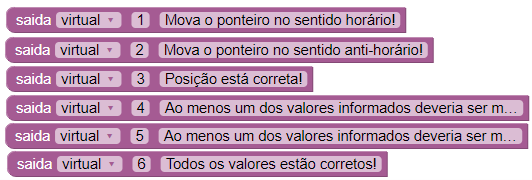
\includegraphics[width=0.8\linewidth]{chapters/appendixC/saidas.png}  \end{tabular}} \\ \hline
	\multicolumn{6}{|c|}{\textbf{JavaScript gerado}} \\ \hline
	\multicolumn{6}{|l|}{\begin{tabular}[c]{@{}l@{}} var SV1 = "Mova o ponteiro no sentido horário!";\\ 			var SV2 = "Mova o ponteiro no sentido anti-horário!";\\ 			var SV3 = "Posição está correta!";\\ 			var SV4 = "Ao menos um dos valores informados deveria ser menor";\\			var SV5 = "Ao menos um dos valores informados deveria ser maior";\\			var SV6 = "Todos os valores estão corretos!"; \end{tabular}} \\ \hline

\end{xltabular}

\begin{xltabular}{\textwidth}{|l|X|}
	\hline
	\endfirsthead
	
	\hline \multicolumn{2}{|c|}{continuação da página anterior} \\ \hline
	\endhead
	
	\hline \multicolumn{2}{|r|}{Continua na próxima página} \\ \hline
	\endfoot
	
	\hline
	\endlastfoot

	\multicolumn{2}{|c|}{\cellcolor[HTML]{C0C0C0}\textbf{CASOS DE TESTE}} \\ \hline

%CASO 1
	\multicolumn{2}{|c|}{\cellcolor[HTML]{DEDEDE}\textbf{CASO DE TESTE 1}} \\ \hline
	\multicolumn{1}{|l|}{\textbf{Rótulo:}} & Dez \\ \hline
	\textbf{Situação-problema (Enunciado):} & Indique o respectivo ângulo e informe seu valor em grau e radiano.\\ \hline
	\multicolumn{2}{|c|}{\cellcolor[HTML]{DEDEDE}\textbf{REGRA 1}} \\ \hline
	\textbf{Blocos} & \multicolumn{1}{c|}{\textbf{JavaScript gerado}} \\ \hline
	\multicolumn{1}{|l|}{\begin{tabular}[c]{@{}l@{}} \\ 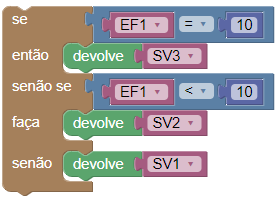
\includegraphics[width=0.4\linewidth]{chapters/appendixC/c1r1.png}  \end{tabular}
	} & \begin{tabular}[c]{@{}l@{}} if((EF1 == 10))\{   return SV3; \} \\ else if ((EF1 \textless 10))\{ return SV2; \} \\ else \{   return SV1; \} \end{tabular} \\ \hline
	\multicolumn{2}{|c|}{\cellcolor[HTML]{DEDEDE}\textbf{REGRA 2}} \\ \hline
	\textbf{Blocos} & \multicolumn{1}{c|}{\textbf{JavaScript gerado}} \\ \hline
	\multicolumn{1}{|l|}{\begin{tabular}[c]{@{}l@{}} \\ 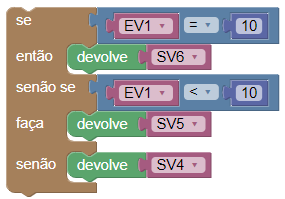
\includegraphics[width=0.4\linewidth]{chapters/appendixC/c1r2.png}  \end{tabular}
	} &  \begin{tabular}[c]{@{}l@{}}if((EV1 == 10))\{   return SV6; \}\\ else if ((EV1 \textless 10))\{ return SV5; \}\\ else \{   return SV4; \} \end{tabular}  \\ \hline
	\multicolumn{2}{|c|}{\cellcolor[HTML]{DEDEDE}\textbf{REGRA 3}} \\ \hline
	\textbf{Blocos} & \multicolumn{1}{c|}{\textbf{JavaScript gerado}} \\ \hline
	\multicolumn{1}{|l|}{\begin{tabular}[c]{@{}l@{}} \\ 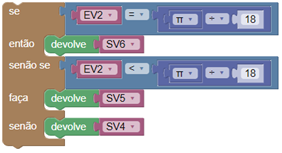
\includegraphics[width=0.4\linewidth]{chapters/appendixC/c1r3.png}  \end{tabular}
	} & if((EV2 == Math.PI / 18))\{   return SV6; \} else if ((EV2 \textless Math.PI / 18))\{   return SV5; \} else \{   return SV4; \} \\ \hline

%CASO 2
		\multicolumn{2}{|c|}{\cellcolor[HTML]{DEDEDE}\textbf{CASO DE TESTE 2}} \\ \hline
		\multicolumn{1}{|l|}{\textbf{Rótulo:}} & Setenta \\ \hline
	\textbf{Situação-problema (Enunciado):} & Indique o respectivo ângulo e informe seu valor em grau e radiano.\\ \hline
		\multicolumn{2}{|c|}{\cellcolor[HTML]{DEDEDE}\textbf{REGRA 1}} \\ \hline
		\textbf{Blocos} & \multicolumn{1}{c|}{\textbf{JavaScript gerado}} \\ \hline
		\multicolumn{1}{|l|}{\begin{tabular}[c]{@{}l@{}} \\ 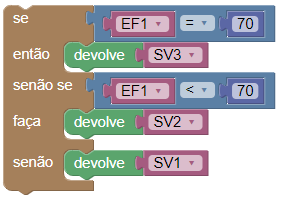
\includegraphics[width=0.4\linewidth]{chapters/appendixC/c2r1.png}  \end{tabular}
		} & \begin{tabular}[c]{@{}l@{}} if((EF1 == 70))\{   return SV3; \}\\ else if ((EF1 \textless 70))\{   return SV2; \}\\ else \{   return SV1; \} \end{tabular} \\ \hline
		\multicolumn{2}{|c|}{\cellcolor[HTML]{DEDEDE}\textbf{REGRA 2}} \\ \hline
		\textbf{Blocos} & \multicolumn{1}{c|}{\textbf{JavaScript gerado}} \\ \hline
		\multicolumn{1}{|l|}{\begin{tabular}[c]{@{}l@{}} \\ 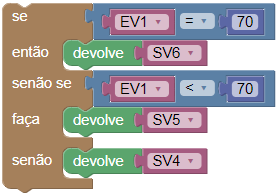
\includegraphics[width=0.4\linewidth]{chapters/appendixC/c2r2.png}  \end{tabular}
		} &  \begin{tabular}[c]{@{}l@{}}if((EV1 == 70))\{   return SV6; \}\\ else if ((EV1 \textless 70))\{   return SV5; \}\\ else \{   return SV4; \} \end{tabular}  \\ \hline
		\multicolumn{2}{|c|}{\cellcolor[HTML]{DEDEDE}\textbf{REGRA 3}} \\ \hline
		\textbf{Blocos} & \multicolumn{1}{c|}{\textbf{JavaScript gerado}} \\ \hline
		\multicolumn{1}{|l|}{\begin{tabular}[c]{@{}l@{}} \\ 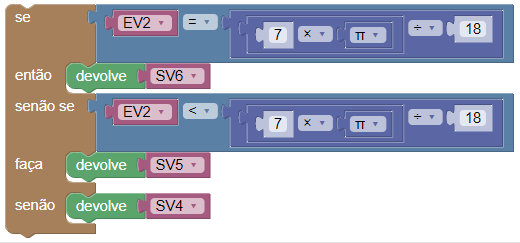
\includegraphics[width=0.4\linewidth]{chapters/appendixC/c2r3.png}  \end{tabular}
		} & if((EV2 == (7 * Math.PI) / 18))\{   return SV6; \} else if ((EV2 \textless (7 * Math.PI) / 18))\{   return SV5; \} else \{   return SV4; \}  \\ \hline

%CASO 3
		\multicolumn{2}{|c|}{\cellcolor[HTML]{DEDEDE}\textbf{CASO DE TESTE 3}} \\ \hline
		\multicolumn{1}{|l|}{\textbf{Rótulo:}} & Trinta \\ \hline
	\textbf{Situação-problema (Enunciado):} & Indique o respectivo ângulo e informe seu valor em grau e radiano.\\ \hline
		\multicolumn{2}{|c|}{\cellcolor[HTML]{DEDEDE}\textbf{REGRA 1}} \\ \hline
		\textbf{Blocos} & \multicolumn{1}{c|}{\textbf{JavaScript gerado}} \\ \hline
		\multicolumn{1}{|l|}{\begin{tabular}[c]{@{}l@{}} \\ 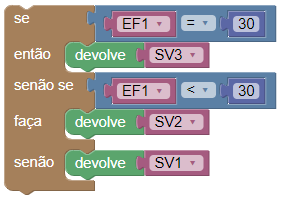
\includegraphics[width=0.4\linewidth]{chapters/appendixC/c3r1.png}  \end{tabular}
		} & \begin{tabular}[c]{@{}l@{}} if((EF1 == 30))\{   return SV3; \}\\ else if ((EF1 \textless 30))\{   return SV2; \}\\ else \{   return SV1; \} \end{tabular} \\ \hline
		\multicolumn{2}{|c|}{\cellcolor[HTML]{DEDEDE}\textbf{REGRA 2}} \\ \hline
		\textbf{Blocos} & \multicolumn{1}{c|}{\textbf{JavaScript gerado}} \\ \hline
		\multicolumn{1}{|l|}{\begin{tabular}[c]{@{}l@{}} \\ 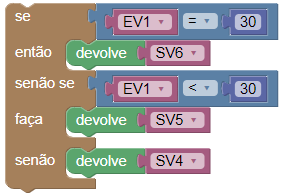
\includegraphics[width=0.4\linewidth]{chapters/appendixC/c3r2.png}  \end{tabular}
		} &  \begin{tabular}[c]{@{}l@{}}if((EV1 == 30))\{   return SV6; \}\\ else if ((EV1 \textless 30))\{   return SV5; \}\\ else \{   return SV4; \} \end{tabular}  \\ \hline
		\multicolumn{2}{|c|}{\cellcolor[HTML]{DEDEDE}\textbf{REGRA 3}} \\ \hline
		\textbf{Blocos} & \multicolumn{1}{c|}{\textbf{JavaScript gerado}} \\ \hline
		\multicolumn{1}{|l|}{\begin{tabular}[c]{@{}l@{}} \\ 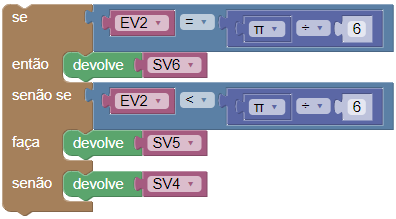
\includegraphics[width=0.4\linewidth]{chapters/appendixC/c3r3.png}  \end{tabular}
		} & if((EV2 == Math.PI / 6))\{   return SV6; \} else if ((EV2 \textless Math.PI / 6))\{   return SV5; \} else \{   return SV4; \} \\ \hline


%CASO 4
		\multicolumn{2}{|c|}{\cellcolor[HTML]{DEDEDE}\textbf{CASO DE TESTE 4}} \\ \hline
		\multicolumn{1}{|l|}{\textbf{Rótulo:}} & $\frac{\pi}{4}$  \\ \hline
	\textbf{Situação-problema (Enunciado):} & Indique o respectivo ângulo e informe seu valor em grau e radiano.\\ \hline
		\multicolumn{2}{|c|}{\cellcolor[HTML]{DEDEDE}\textbf{REGRA 1}} \\ \hline
		\textbf{Blocos} & \multicolumn{1}{c|}{\textbf{JavaScript gerado}} \\ \hline
		\multicolumn{1}{|l|}{\begin{tabular}[c]{@{}l@{}} \\ 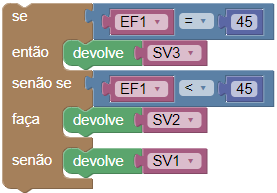
\includegraphics[width=0.4\linewidth]{chapters/appendixC/c4r1.png}  \end{tabular}
		} & \begin{tabular}[c]{@{}l@{}} if((EF1 == 45))\{   return SV3; \}\\ else if ((EF1 \textless 45))\{   return SV2; \}\\ else \{   return SV1; \} \end{tabular} \\ \hline
		\multicolumn{2}{|c|}{\cellcolor[HTML]{DEDEDE}\textbf{REGRA 2}} \\ \hline
		\textbf{Blocos} & \multicolumn{1}{c|}{\textbf{JavaScript gerado}} \\ \hline
		\multicolumn{1}{|l|}{\begin{tabular}[c]{@{}l@{}} \\ 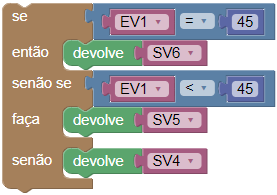
\includegraphics[width=0.4\linewidth]{chapters/appendixC/c4r2.png}  \end{tabular}
		} &  \begin{tabular}[c]{@{}l@{}}if((EV1 == 45))\{   return SV6; \}\\ else if ((EV1 \textless 45))\{   return SV5; \}\\ else \{   return SV4; \} \end{tabular}  \\ \hline
		\multicolumn{2}{|c|}{\cellcolor[HTML]{DEDEDE}\textbf{REGRA 3}} \\ \hline
		\textbf{Blocos} & \multicolumn{1}{c|}{\textbf{JavaScript gerado}} \\ \hline
		\multicolumn{1}{|l|}{\begin{tabular}[c]{@{}l@{}} \\ 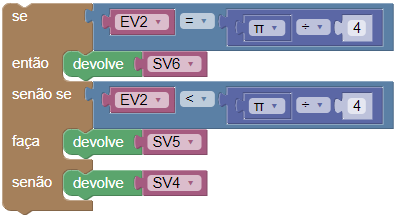
\includegraphics[width=0.4\linewidth]{chapters/appendixC/c4r3.png}  \end{tabular}
		} & if((EV2 == Math.PI / 4))\{   return SV6; \} else if ((EV2 \textless Math.PI / 4))\{   return SV5; \} else \{   return SV4; \} \\ \hline

%CASO 5
		\multicolumn{2}{|c|}{\cellcolor[HTML]{DEDEDE}\textbf{CASO DE TESTE 5}} \\ \hline
		\multicolumn{1}{|l|}{\textbf{Rótulo:}} & $120$  \\ \hline
	\textbf{Situação-problema (Enunciado):} & Indique o respectivo ângulo e informe seu valor em grau e radiano.\\ \hline
		\multicolumn{2}{|c|}{\cellcolor[HTML]{DEDEDE}\textbf{REGRA 1}} \\ \hline
		\textbf{Blocos} & \multicolumn{1}{c|}{\textbf{JavaScript gerado}} \\ \hline
		\multicolumn{1}{|l|}{\begin{tabular}[c]{@{}l@{}} \\ 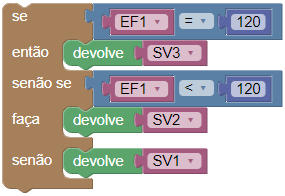
\includegraphics[width=0.4\linewidth]{chapters/appendixC/c5r1.png}  \end{tabular}
		} & \begin{tabular}[c]{@{}l@{}} if((EF1 == 120))\{   return SV3; \}\\ else if ((EF1 \textless 120))\{   return SV2; \}\\ else \{   return SV1; \} \end{tabular} \\ \hline
		\multicolumn{2}{|c|}{\cellcolor[HTML]{DEDEDE}\textbf{REGRA 2}} \\ \hline
		\textbf{Blocos} & \multicolumn{1}{c|}{\textbf{JavaScript gerado}} \\ \hline
		\multicolumn{1}{|l|}{\begin{tabular}[c]{@{}l@{}} \\ 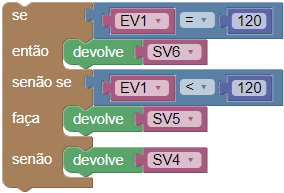
\includegraphics[width=0.4\linewidth]{chapters/appendixC/c5r2.png}  \end{tabular}
		} &  \begin{tabular}[c]{@{}l@{}}if((EV1 == 120))\{   return SV6; \}\\ else if ((EV1 \textless 120))\{   return SV5; \}\\ else \{   return SV4; \} \end{tabular}  \\ \hline
		\multicolumn{2}{|c|}{\cellcolor[HTML]{DEDEDE}\textbf{REGRA 3}} \\ \hline
		\textbf{Blocos} & \multicolumn{1}{c|}{\textbf{JavaScript gerado}} \\ \hline
		\multicolumn{1}{|l|}{\begin{tabular}[c]{@{}l@{}} \\ 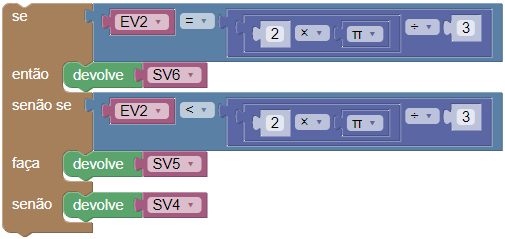
\includegraphics[width=0.4\linewidth]{chapters/appendixC/c5r3.png}  \end{tabular}
		} & if((EV2 == (2 * Math.PI) / 3))\{   return SV6; \} else if ((EV2 \textless (2 * Math.PI) / 3))\{   return SV5; \} else \{   return SV4; \} \\ \hline

%CASO 6
		\multicolumn{2}{|c|}{\cellcolor[HTML]{DEDEDE}\textbf{CASO DE TESTE 6}} \\ \hline
		\multicolumn{1}{|l|}{\textbf{Rótulo:}} & $150$  \\ \hline
	\textbf{Situação-problema (Enunciado):} & Indique o respectivo ângulo e informe seu valor em grau e radiano.\\ \hline
		\multicolumn{2}{|c|}{\cellcolor[HTML]{DEDEDE}\textbf{REGRA 1}} \\ \hline
		\textbf{Blocos} & \multicolumn{1}{c|}{\textbf{JavaScript gerado}} \\ \hline
		\multicolumn{1}{|l|}{\begin{tabular}[c]{@{}l@{}} \\ 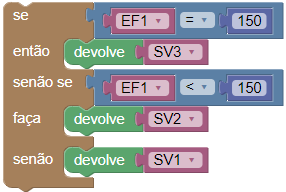
\includegraphics[width=0.4\linewidth]{chapters/appendixC/c6r1.png}  \end{tabular}
		} & \begin{tabular}[c]{@{}l@{}} if((EF1 == 150))\{   return SV3; \}\\ else if ((EF1 < 150))\{   return SV2; \}\\ else \{   return SV1; \} \end{tabular} \\ \hline
		\multicolumn{2}{|c|}{\cellcolor[HTML]{DEDEDE}\textbf{REGRA 2}} \\ \hline
		\textbf{Blocos} & \multicolumn{1}{c|}{\textbf{JavaScript gerado}} \\ \hline
		\multicolumn{1}{|l|}{\begin{tabular}[c]{@{}l@{}} \\ 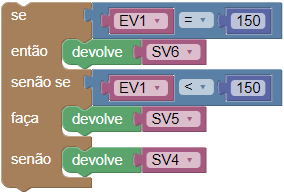
\includegraphics[width=0.4\linewidth]{chapters/appendixC/c6r2.png}  \end{tabular}
		} &  \begin{tabular}[c]{@{}l@{}}if((EV1 == 150))\{   return SV6; \}\\ else if ((EV1 < 150))\{   return SV5; \}\\ else \{   return SV4; \} \end{tabular}  \\ \hline
		\multicolumn{2}{|c|}{\cellcolor[HTML]{DEDEDE}\textbf{REGRA 3}} \\ \hline
		\textbf{Blocos} & \multicolumn{1}{c|}{\textbf{JavaScript gerado}} \\ \hline
		\multicolumn{1}{|l|}{\begin{tabular}[c]{@{}l@{}} \\ 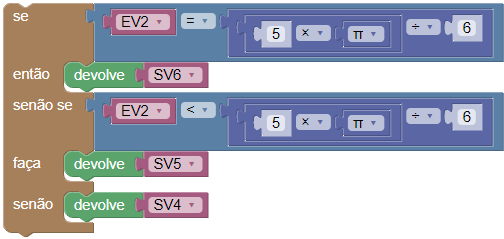
\includegraphics[width=0.4\linewidth]{chapters/appendixC/c6r3.png}  \end{tabular}
		} & if((EV2 == (5 * Math.PI) / 6))\{   return SV6; \} else if ((EV2 < (5 * Math.PI) / 6))\{   return SV5; \} else \{   return SV4; \} \\ \hline

%CASO 7
		\multicolumn{2}{|c|}{\cellcolor[HTML]{DEDEDE}\textbf{CASO DE TESTE 7}} \\ \hline
		\multicolumn{1}{|l|}{\textbf{Rótulo:}} & $\frac{3 \pi}{4}$  \\ \hline
	\textbf{Situação-problema (Enunciado):} & Indique o respectivo ângulo e informe seu valor em grau e radiano.\\ \hline
		\multicolumn{2}{|c|}{\cellcolor[HTML]{DEDEDE}\textbf{REGRA 1}} \\ \hline
		\textbf{Blocos} & \multicolumn{1}{c|}{\textbf{JavaScript gerado}} \\ \hline
		\multicolumn{1}{|l|}{\begin{tabular}[c]{@{}l@{}} \\ 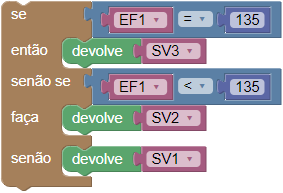
\includegraphics[width=0.4\linewidth]{chapters/appendixC/c7r1.png}  \end{tabular}
		} & \begin{tabular}[c]{@{}l@{}} if((EF1 == 135))\{   return SV3; \}\\ else if ((EF1 < 135))\{   return SV2; \}\\ else \{   return SV1; \} \end{tabular} \\ \hline
		\multicolumn{2}{|c|}{\cellcolor[HTML]{DEDEDE}\textbf{REGRA 2}} \\ \hline
		\textbf{Blocos} & \multicolumn{1}{c|}{\textbf{JavaScript gerado}} \\ \hline
		\multicolumn{1}{|l|}{\begin{tabular}[c]{@{}l@{}} \\ 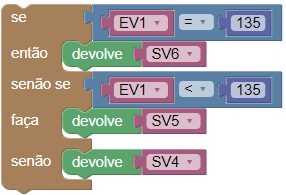
\includegraphics[width=0.4\linewidth]{chapters/appendixC/c7r2.png}  \end{tabular}
		} &  \begin{tabular}[c]{@{}l@{}}if((EV1 == 135))\{   return SV6; \}\\ else if ((EV1 < 135))\{   return SV5; \}\\ else \{   return SV4; \} \end{tabular}  \\ \hline
		\multicolumn{2}{|c|}{\cellcolor[HTML]{DEDEDE}\textbf{REGRA 3}} \\ \hline
		\textbf{Blocos} & \multicolumn{1}{c|}{\textbf{JavaScript gerado}} \\ \hline
		\multicolumn{1}{|l|}{\begin{tabular}[c]{@{}l@{}} \\ 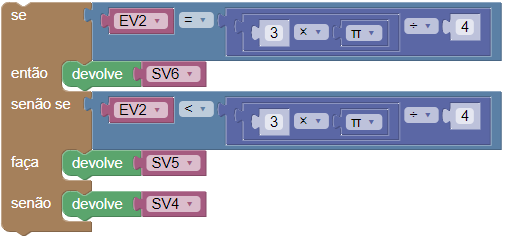
\includegraphics[width=0.4\linewidth]{chapters/appendixC/c7r3.png}  \end{tabular}
		} & if((EV2 == (3 * Math.PI) / 4))\{   return SV6; \} else if ((EV2 < (3 * Math.PI) / 4))\{   return SV5; \} else \{   return SV4; \} \\ \hline


%CASO 8
		\multicolumn{2}{|c|}{\cellcolor[HTML]{DEDEDE}\textbf{CASO DE TESTE 8}} \\ \hline
		\multicolumn{1}{|l|}{\textbf{Rótulo:}} & $\frac{7 \pi}{6}$  \\ \hline
	\textbf{Situação-problema (Enunciado):} & Indique o respectivo ângulo e informe seu valor em grau e radiano.\\ \hline
		\multicolumn{2}{|c|}{\cellcolor[HTML]{DEDEDE}\textbf{REGRA 1}} \\ \hline
		\textbf{Blocos} & \multicolumn{1}{c|}{\textbf{JavaScript gerado}} \\ \hline
		\multicolumn{1}{|l|}{\begin{tabular}[c]{@{}l@{}} \\ 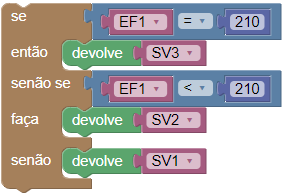
\includegraphics[width=0.4\linewidth]{chapters/appendixC/c8r1.png}  \end{tabular}
		} & \begin{tabular}[c]{@{}l@{}} if((EF1 == 210))\{   return SV3; \}\\ else if ((EF1 < 210))\{   return SV2; \}\\else \{   return SV1; \} \end{tabular} \\ \hline
		\multicolumn{2}{|c|}{\cellcolor[HTML]{DEDEDE}\textbf{REGRA 2}} \\ \hline
		\textbf{Blocos} & \multicolumn{1}{c|}{\textbf{JavaScript gerado}} \\ \hline
		\multicolumn{1}{|l|}{\begin{tabular}[c]{@{}l@{}} \\ 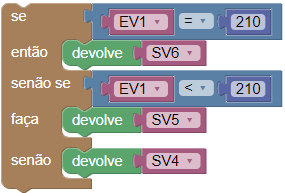
\includegraphics[width=0.4\linewidth]{chapters/appendixC/c8r2.png}  \end{tabular}
		} &  \begin{tabular}[c]{@{}l@{}}if((EV1 == 210))\{   return SV6; \}\\ else if ((EV1 < 210))\{   return SV5; \}\\ else \{   return SV4; \} \end{tabular}  \\ \hline
		\multicolumn{2}{|c|}{\cellcolor[HTML]{DEDEDE}\textbf{REGRA 3}} \\ \hline
		\textbf{Blocos} & \multicolumn{1}{c|}{\textbf{JavaScript gerado}} \\ \hline
		\multicolumn{1}{|l|}{\begin{tabular}[c]{@{}l@{}} \\ 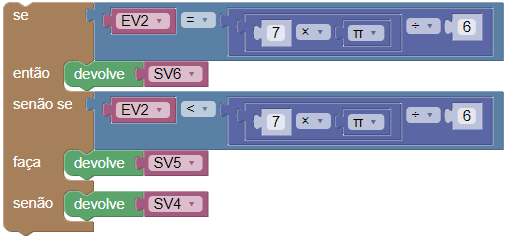
\includegraphics[width=0.4\linewidth]{chapters/appendixC/c8r3.png}  \end{tabular}
		} & if((EV2 == (7 * Math.PI) / 6))\{   return SV6; \} else if ((EV2 < (7 * Math.PI) / 6))\{   return SV5; \} else \{   return SV4; \} \\ \hline


%CASO 9
 		\multicolumn{2}{|c|}{\cellcolor[HTML]{DEDEDE}\textbf{CASO DE TESTE 9}} \\ \hline
		\multicolumn{1}{|l|}{\textbf{Rótulo:}} & $240$  \\ \hline
	\textbf{Situação-problema (Enunciado):} & Indique o respectivo ângulo e informe seu valor em grau e radiano.\\ \hline
		\multicolumn{2}{|c|}{\cellcolor[HTML]{DEDEDE}\textbf{REGRA 1}} \\ \hline
		\textbf{Blocos} & \multicolumn{1}{c|}{\textbf{JavaScript gerado}} \\ \hline
		\multicolumn{1}{|l|}{\begin{tabular}[c]{@{}l@{}} \\ 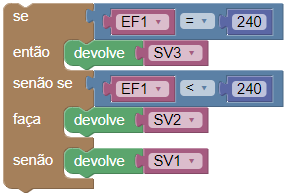
\includegraphics[width=0.4\linewidth]{chapters/appendixC/c9r1.png}  \end{tabular}
		} & \begin{tabular}[c]{@{}l@{}} if((EF1 == 240))\{   return SV3; \}\\ else if ((EF1 < 240))\{   return SV2; \}\\ else \{   return SV1; \} \end{tabular} \\ \hline
		\multicolumn{2}{|c|}{\cellcolor[HTML]{DEDEDE}\textbf{REGRA 2}} \\ \hline
		\textbf{Blocos} & \multicolumn{1}{c|}{\textbf{JavaScript gerado}} \\ \hline
		\multicolumn{1}{|l|}{\begin{tabular}[c]{@{}l@{}} \\ 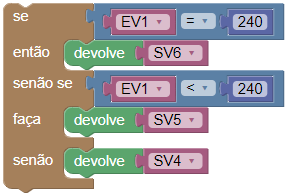
\includegraphics[width=0.4\linewidth]{chapters/appendixC/c9r2.png}  \end{tabular}
		} &  \begin{tabular}[c]{@{}l@{}}if((EV1 == 240))\{   return SV6; \}\\ else if ((EV1 < 240))\{   return SV5; \}\\ else \{   return SV4; \} \end{tabular}  \\ \hline
		\multicolumn{2}{|c|}{\cellcolor[HTML]{DEDEDE}\textbf{REGRA 3}} \\ \hline
		\textbf{Blocos} & \multicolumn{1}{c|}{\textbf{JavaScript gerado}} \\ \hline
		\multicolumn{1}{|l|}{\begin{tabular}[c]{@{}l@{}} \\ 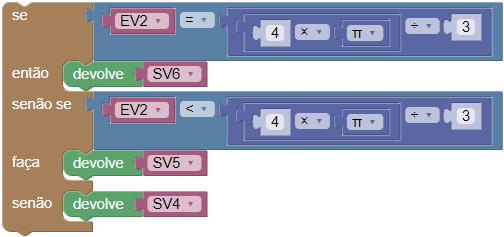
\includegraphics[width=0.4\linewidth]{chapters/appendixC/c9r3.png}  \end{tabular}
		} & if((EV2 == (4 * Math.PI) / 3))\{   return SV6; \} else if ((EV2 < (4 * Math.PI) / 3))\{   return SV5; \} else \{   return SV4; \} \\ \hline


%CASO 10
		\multicolumn{2}{|c|}{\cellcolor[HTML]{DEDEDE}\textbf{CASO DE TESTE 10}} \\ \hline
		\multicolumn{1}{|l|}{\textbf{Rótulo:}} & $\frac{5 \pi}{3}$  \\ \hline
	\textbf{Situação-problema (Enunciado):} & Indique o respectivo ângulo e informe seu valor em grau e radiano.\\ \hline
		\multicolumn{2}{|c|}{\cellcolor[HTML]{DEDEDE}\textbf{REGRA 1}} \\ \hline
		\textbf{Blocos} & \multicolumn{1}{c|}{\textbf{JavaScript gerado}} \\ \hline
		\multicolumn{1}{|l|}{\begin{tabular}[c]{@{}l@{}} \\ 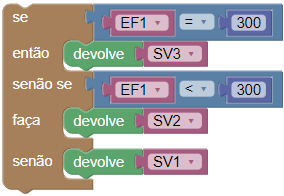
\includegraphics[width=0.4\linewidth]{chapters/appendixC/c10r1.png}  \end{tabular}
		} & \begin{tabular}[c]{@{}l@{}} if((EF1 == 300))\{   return SV3; \}\\ else if ((EF1 < 300))\{   return SV2; \}\\ else \{   return SV1; \} \end{tabular} \\ \hline
		\multicolumn{2}{|c|}{\cellcolor[HTML]{DEDEDE}\textbf{REGRA 2}} \\ \hline
		\textbf{Blocos} & \multicolumn{1}{c|}{\textbf{JavaScript gerado}} \\ \hline
		\multicolumn{1}{|l|}{\begin{tabular}[c]{@{}l@{}} \\ 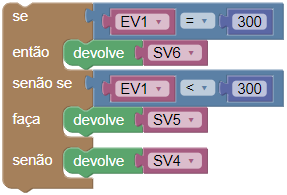
\includegraphics[width=0.4\linewidth]{chapters/appendixC/c10r2.png}  \end{tabular}
		} &  \begin{tabular}[c]{@{}l@{}}if((EV1 == 300))\{   return SV6; \}\\ else if ((EV1 < 300))\{   return SV5; \}\\ else \{   return SV4; \} \end{tabular}  \\ \hline
		\multicolumn{2}{|c|}{\cellcolor[HTML]{DEDEDE}\textbf{REGRA 3}} \\ \hline
		\textbf{Blocos} & \multicolumn{1}{c|}{\textbf{JavaScript gerado}} \\ \hline
		\multicolumn{1}{|l|}{\begin{tabular}[c]{@{}l@{}} \\ 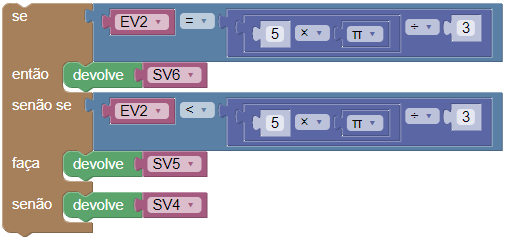
\includegraphics[width=0.4\linewidth]{chapters/appendixC/c10r3.png}  \end{tabular}
		} & if((EV2 == (5 * Math.PI) / 3))\{   return SV6; \} else if ((EV2 < (5 * Math.PI) / 3))\{   return SV5; \} else \{   return SV4; \} \\ \hline


%CASO 11
		\multicolumn{2}{|c|}{\cellcolor[HTML]{DEDEDE}\textbf{CASO DE TESTE 11}} \\ \hline
		\multicolumn{1}{|l|}{\textbf{Rótulo:}} & $330$  \\ \hline
	\textbf{Situação-problema (Enunciado):} & Indique o respectivo ângulo e informe seu valor em grau e radiano.\\ \hline
		\multicolumn{2}{|c|}{\cellcolor[HTML]{DEDEDE}\textbf{REGRA 1}} \\ \hline
		\textbf{Blocos} & \multicolumn{1}{c|}{\textbf{JavaScript gerado}} \\ \hline
		\multicolumn{1}{|l|}{\begin{tabular}[c]{@{}l@{}} \\ 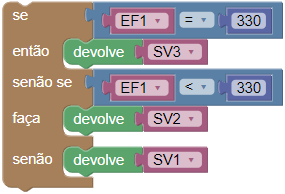
\includegraphics[width=0.4\linewidth]{chapters/appendixC/c11r1.png}  \end{tabular}
		} & \begin{tabular}[c]{@{}l@{}} if((EF1 == 330))\{   return SV3; \}\\ else if ((EF1 < 330))\{   return SV2; \}\\ else \{   return SV1; \} \end{tabular} \\ \hline
		\multicolumn{2}{|c|}{\cellcolor[HTML]{DEDEDE}\textbf{REGRA 2}} \\ \hline
		\textbf{Blocos} & \multicolumn{1}{c|}{\textbf{JavaScript gerado}} \\ \hline
		\multicolumn{1}{|l|}{\begin{tabular}[c]{@{}l@{}} \\ 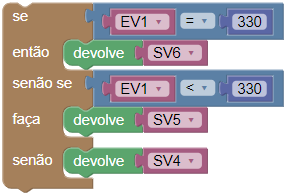
\includegraphics[width=0.4\linewidth]{chapters/appendixC/c11r2.png}  \end{tabular}
		} &  \begin{tabular}[c]{@{}l@{}}if((EV1 == 330))\{   return SV6; \}\\ else if ((EV1 < 330))\{   return SV5; \}\\ else \{   return SV4; \} \end{tabular}  \\ \hline
		\multicolumn{2}{|c|}{\cellcolor[HTML]{DEDEDE}\textbf{REGRA 3}} \\ \hline
		\textbf{Blocos} & \multicolumn{1}{c|}{\textbf{JavaScript gerado}} \\ \hline
		\multicolumn{1}{|l|}{\begin{tabular}[c]{@{}l@{}} \\ 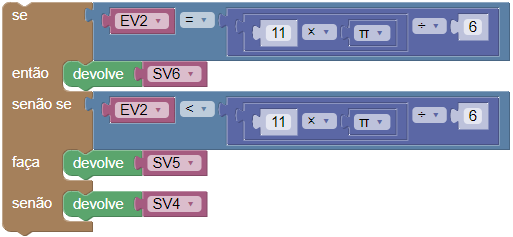
\includegraphics[width=0.4\linewidth]{chapters/appendixC/c11r3.png}  \end{tabular}
		} & if((EV2 == (11 * Math.PI) / 6))\{   return SV6; \} else if ((EV2 < (11 * Math.PI) / 6))\{   return SV5; \} else \{   return SV4; \} \\ \hline


%CASO 12
		\multicolumn{2}{|c|}{\cellcolor[HTML]{DEDEDE}\textbf{CASO DE TESTE 12}} \\ \hline
		\multicolumn{1}{|l|}{\textbf{Rótulo:}} & $420$  \\ \hline
	\textbf{Situação-problema (Enunciado):} & Indique o respectivo ângulo e informe seu valor em grau e radiano.\\ \hline
		\multicolumn{2}{|c|}{\cellcolor[HTML]{DEDEDE}\textbf{REGRA 1}} \\ \hline
		\textbf{Blocos} & \multicolumn{1}{c|}{\textbf{JavaScript gerado}} \\ \hline
		\multicolumn{1}{|l|}{\begin{tabular}[c]{@{}l@{}} \\ 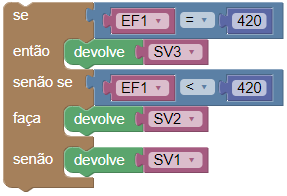
\includegraphics[width=0.4\linewidth]{chapters/appendixC/c12r1.png}  \end{tabular}
		} & \begin{tabular}[c]{@{}l@{}} if((EF1 == 420))\{   return SV3; \}\\ else if ((EF1 < 420))\{   return SV2; \}\\ else \{   return SV1; \} \end{tabular} \\ \hline
		\multicolumn{2}{|c|}{\cellcolor[HTML]{DEDEDE}\textbf{REGRA 2}} \\ \hline
		\textbf{Blocos} & \multicolumn{1}{c|}{\textbf{JavaScript gerado}} \\ \hline
		\multicolumn{1}{|l|}{\begin{tabular}[c]{@{}l@{}} \\ 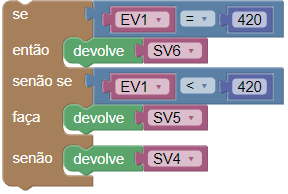
\includegraphics[width=0.4\linewidth]{chapters/appendixC/c12r2.png}  \end{tabular}
		} &  \begin{tabular}[c]{@{}l@{}}if((EV1 == 420))\{   return SV6; \}\\ else if ((EV1 < 420))\{   return SV5; \}\\ else \{   return SV4; \} \end{tabular}  \\ \hline
		\multicolumn{2}{|c|}{\cellcolor[HTML]{DEDEDE}\textbf{REGRA 3}} \\ \hline
		\textbf{Blocos} & \multicolumn{1}{c|}{\textbf{JavaScript gerado}} \\ \hline
		\multicolumn{1}{|l|}{\begin{tabular}[c]{@{}l@{}} \\ 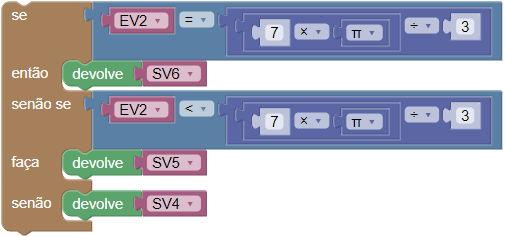
\includegraphics[width=0.4\linewidth]{chapters/appendixC/c12r3.png}  \end{tabular}
		} & if((EV2 == (7 * Math.PI) / 3))\{   return SV6; \} else if ((EV2 < (7 * Math.PI) / 3))\{   return SV5; \} else \{   return SV4; \} \\ \hline


%CASO 13
		\multicolumn{2}{|c|}{\cellcolor[HTML]{DEDEDE}\textbf{CASO DE TESTE 13}} \\ \hline
		\multicolumn{1}{|l|}{\textbf{Rótulo:}} & $480$  \\ \hline
	\textbf{Situação-problema (Enunciado):} & Indique o respectivo ângulo e informe seu valor em grau e radiano.\\ \hline
		\multicolumn{2}{|c|}{\cellcolor[HTML]{DEDEDE}\textbf{REGRA 1}} \\ \hline
		\textbf{Blocos} & \multicolumn{1}{c|}{\textbf{JavaScript gerado}} \\ \hline
		\multicolumn{1}{|l|}{\begin{tabular}[c]{@{}l@{}} \\ 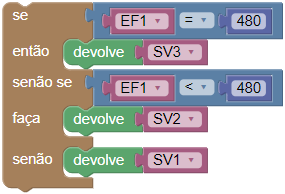
\includegraphics[width=0.4\linewidth]{chapters/appendixC/c13r1.png}  \end{tabular}
		} & \begin{tabular}[c]{@{}l@{}} if((EF1 == 480))\{   return SV3; \}\\ else if ((EF1 < 480))\{   return SV2; \}\\ else \{   return SV1; \} \end{tabular} \\ \hline
		\multicolumn{2}{|c|}{\cellcolor[HTML]{DEDEDE}\textbf{REGRA 2}} \\ \hline
		\textbf{Blocos} & \multicolumn{1}{c|}{\textbf{JavaScript gerado}} \\ \hline
		\multicolumn{1}{|l|}{\begin{tabular}[c]{@{}l@{}} \\ 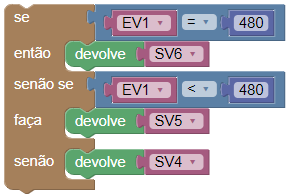
\includegraphics[width=0.4\linewidth]{chapters/appendixC/c13r2.png}  \end{tabular}
		} &  \begin{tabular}[c]{@{}l@{}}if((EV1 == 480))\{   return SV6; \}\\ else if ((EV1 < 480))\{   return SV5; \}\\ else \{   return SV4; \} \end{tabular}  \\ \hline
		\multicolumn{2}{|c|}{\cellcolor[HTML]{DEDEDE}\textbf{REGRA 3}} \\ \hline
		\textbf{Blocos} & \multicolumn{1}{c|}{\textbf{JavaScript gerado}} \\ \hline
		\multicolumn{1}{|l|}{\begin{tabular}[c]{@{}l@{}} \\ 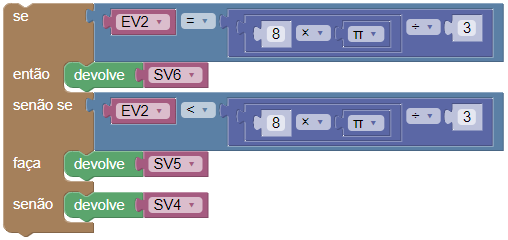
\includegraphics[width=0.4\linewidth]{chapters/appendixC/c13r3.png}  \end{tabular}
		} & if((EV2 == (8 * Math.PI) / 3))\{   return SV6; \} else if ((EV2 < (8 * Math.PI) / 3))\{   return SV5; \} else \{   return SV4; \} \\ \hline


%CASO 14
		\multicolumn{2}{|c|}{\cellcolor[HTML]{DEDEDE}\textbf{CASO DE TESTE 14}} \\ \hline
		\multicolumn{1}{|l|}{\textbf{Rótulo:}} & $540$  \\ \hline
	\textbf{Situação-problema (Enunciado):} & Indique o respectivo ângulo e informe seu valor em grau e radiano.\\ \hline
		\multicolumn{2}{|c|}{\cellcolor[HTML]{DEDEDE}\textbf{REGRA 1}} \\ \hline
		\textbf{Blocos} & \multicolumn{1}{c|}{\textbf{JavaScript gerado}} \\ \hline
		\multicolumn{1}{|l|}{\begin{tabular}[c]{@{}l@{}} \\ 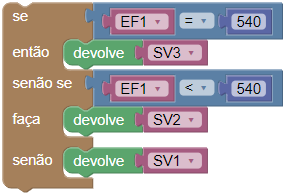
\includegraphics[width=0.4\linewidth]{chapters/appendixC/c14r1.png}  \end{tabular}
		} & \begin{tabular}[c]{@{}l@{}} if((EF1 == 540))\{   return SV3; \}\\ else if ((EF1 < 540))\{   return SV2; \}\\ else \{   return SV1; \} \end{tabular} \\ \hline
		\multicolumn{2}{|c|}{\cellcolor[HTML]{DEDEDE}\textbf{REGRA 2}} \\ \hline
		\textbf{Blocos} & \multicolumn{1}{c|}{\textbf{JavaScript gerado}} \\ \hline
		\multicolumn{1}{|l|}{\begin{tabular}[c]{@{}l@{}} \\ 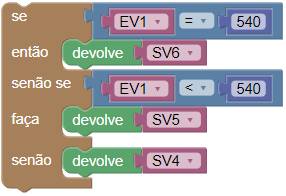
\includegraphics[width=0.4\linewidth]{chapters/appendixC/c14r2.png}  \end{tabular}
		} &  \begin{tabular}[c]{@{}l@{}}if((EV1 == 540))\{   return SV6; \}\\ else if ((EV1 < 540))\{   return SV5; \}\\ else \{   return SV4; \} \end{tabular}  \\ \hline
		\multicolumn{2}{|c|}{\cellcolor[HTML]{DEDEDE}\textbf{REGRA 3}} \\ \hline
		\textbf{Blocos} & \multicolumn{1}{c|}{\textbf{JavaScript gerado}} \\ \hline
		\multicolumn{1}{|l|}{\begin{tabular}[c]{@{}l@{}} \\ 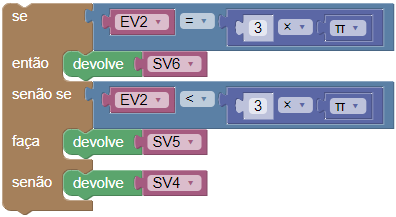
\includegraphics[width=0.4\linewidth]{chapters/appendixC/c14r3.png}  \end{tabular}
		} & if((EV2 == 3 * Math.PI))\{   return SV6; \} else if ((EV2 < 3 * Math.PI))\{   return SV5; \} else \{   return SV4; \} \\ \hline


%CASO 15
		\multicolumn{2}{|c|}{\cellcolor[HTML]{DEDEDE}\textbf{CASO DE TESTE 15}} \\ \hline
		\multicolumn{1}{|l|}{\textbf{Rótulo:}} & $600$  \\ \hline
	\textbf{Situação-problema (Enunciado):} & Indique o respectivo ângulo e informe seu valor em grau e radiano.\\ \hline
		\multicolumn{2}{|c|}{\cellcolor[HTML]{DEDEDE}\textbf{REGRA 1}} \\ \hline
		\textbf{Blocos} & \multicolumn{1}{c|}{\textbf{JavaScript gerado}} \\ \hline
		\multicolumn{1}{|l|}{\begin{tabular}[c]{@{}l@{}} \\ 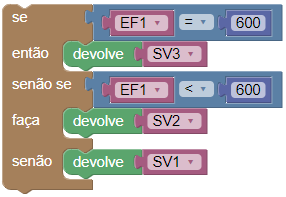
\includegraphics[width=0.4\linewidth]{chapters/appendixC/c15r1.png}  \end{tabular}
		} & \begin{tabular}[c]{@{}l@{}} if((EF1 == 600))\{   return SV3; \}\\ else if ((EF1 < 600))\{   return SV2; \}\\ else \{   return SV1; \} \end{tabular} \\ \hline
		\multicolumn{2}{|c|}{\cellcolor[HTML]{DEDEDE}\textbf{REGRA 2}} \\ \hline
		\textbf{Blocos} & \multicolumn{1}{c|}{\textbf{JavaScript gerado}} \\ \hline
		\multicolumn{1}{|l|}{\begin{tabular}[c]{@{}l@{}} \\ 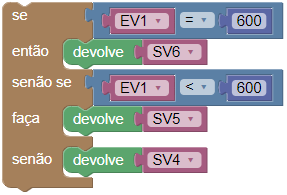
\includegraphics[width=0.4\linewidth]{chapters/appendixC/c15r2.png}  \end{tabular}
		} &  \begin{tabular}[c]{@{}l@{}}if((EV1 == 600))\{   return SV6; \}\\ else if ((EV1 < 600))\{   return SV5; \}\\ else \{   return SV4; \} \end{tabular}  \\ \hline
		\multicolumn{2}{|c|}{\cellcolor[HTML]{DEDEDE}\textbf{REGRA 3}} \\ \hline
		\textbf{Blocos} & \multicolumn{1}{c|}{\textbf{JavaScript gerado}} \\ \hline
		\multicolumn{1}{|l|}{\begin{tabular}[c]{@{}l@{}} \\ 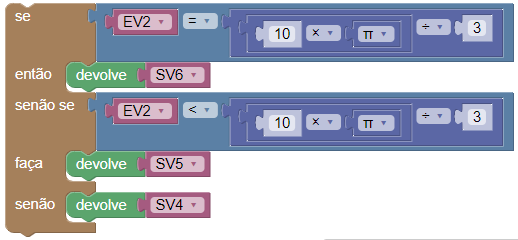
\includegraphics[width=0.4\linewidth]{chapters/appendixC/c15r3.png}  \end{tabular}
		} & if((EV2 == (10 * Math.PI) / 3))\{   return SV6; \} else if ((EV2 < (10 * Math.PI) / 3))\{   return SV5; \} else \{   return SV4; \} \\ \hline


%CASO 16
%		\multicolumn{2}{|c|}{\cellcolor[HTML]{DEDEDE}\textbf{CASO DE TESTE 16}} \\ \hline
%		\multicolumn{1}{|l|}{\textbf{Rótulo:}} & $600$  \\ \hline
%	\textbf{Situação-problema (Enunciado):} & Indique o respectivo ângulo e informe seu valor em grau e radiano.\\ \hline
%		\multicolumn{2}{|c|}{\cellcolor[HTML]{DEDEDE}\textbf{REGRA 1}} \\ \hline
%		\textbf{Blocos} & \multicolumn{1}{c|}{\textbf{JavaScript gerado}} \\ \hline
%		\multicolumn{1}{|l|}{\begin{tabular}[c]{@{}l@{}} \\ 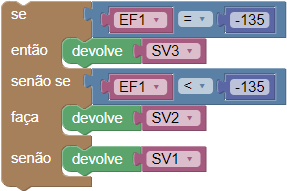
\includegraphics[width=0.4\linewidth]{chapters/appendixC/c16r1.png}  \end{tabular}
%		} & \begin{tabular}[c]{@{}l@{}} if((EF1 == 600))\{   return SV3; \}\\ else if ((EF1 < 600))\{   return SV2; \}\\ else \{   return SV1; \} \end{tabular} \\ \hline
%		\multicolumn{2}{|c|}{\cellcolor[HTML]{DEDEDE}\textbf{REGRA 2}} \\ \hline
%		\textbf{Blocos} & \multicolumn{1}{c|}{\textbf{JavaScript gerado}} \\ \hline
%		\multicolumn{1}{|l|}{\begin{tabular}[c]{@{}l@{}} \\ \includegraphics[width=0.4\linewidth]{chapters/appendixC/c16r2.png}  \end{tabular}
%		} &  \begin{tabular}[c]{@{}l@{}}if((EV1 == 600))\{   return SV6; \}\\ else if ((EV1 < 600))\{   return SV5; \}\\ else \{   return SV4; \} \end{tabular}  \\ \hline
%		\multicolumn{2}{|c|}{\cellcolor[HTML]{DEDEDE}\textbf{REGRA 3}} \\ \hline
%		\textbf{Blocos} & \multicolumn{1}{c|}{\textbf{JavaScript gerado}} \\ \hline
%		\multicolumn{1}{|l|}{\begin{tabular}[c]{@{}l@{}} \\ \includegraphics[width=0.4\linewidth]{chapters/appendixC/c16r3.png}  \end{tabular}
%		} & if((EV2 == (10 * Math.PI) / 3))\{   return SV6; \} else if ((EV2 < (10 * Math.PI) / 3))\{   return SV5; \} else \{   return SV4; \} \\ \hline


%CASO 16
		\multicolumn{2}{|c|}{\cellcolor[HTML]{DEDEDE}\textbf{CASO DE TESTE 16}} \\ \hline
		\multicolumn{1}{|l|}{\textbf{Rótulo:}} & $-135$  \\ \hline
	\textbf{Situação-problema (Enunciado):} & Indique o respectivo ângulo e informe seu valor em grau e radiano.\\ \hline
		\multicolumn{2}{|c|}{\cellcolor[HTML]{DEDEDE}\textbf{REGRA 1}} \\ \hline
		\textbf{Blocos} & \multicolumn{1}{c|}{\textbf{JavaScript gerado}} \\ \hline
		\multicolumn{1}{|l|}{\begin{tabular}[c]{@{}l@{}} \\ \includegraphics[width=0.4\linewidth]{chapters/appendixC/c17r1.png}  \end{tabular}
		} & \begin{tabular}[c]{@{}l@{}} if((EF1 == -135))\{   return SV3; \}\\ else if ((EF1 < -135))\{   return SV2; \}\\ else \{   return SV1; \} \end{tabular} \\ \hline
		\multicolumn{2}{|c|}{\cellcolor[HTML]{DEDEDE}\textbf{REGRA 2}} \\ \hline
		\textbf{Blocos} & \multicolumn{1}{c|}{\textbf{JavaScript gerado}} \\ \hline
		\multicolumn{1}{|l|}{\begin{tabular}[c]{@{}l@{}} \\ \includegraphics[width=0.4\linewidth]{chapters/appendixC/c17r2.png}  \end{tabular}
		} &  \begin{tabular}[c]{@{}l@{}}if((EV1 == -135))\{   return SV6; \}\\ else if ((EV1 < -135))\{   return SV5; \}\\ else \{   return SV4; \} \end{tabular}  \\ \hline
		\multicolumn{2}{|c|}{\cellcolor[HTML]{DEDEDE}\textbf{REGRA 3}} \\ \hline
		\textbf{Blocos} & \multicolumn{1}{c|}{\textbf{JavaScript gerado}} \\ \hline
		\multicolumn{1}{|l|}{\begin{tabular}[c]{@{}l@{}} \\ \includegraphics[width=0.4\linewidth]{chapters/appendixC/c17r3.png}  \end{tabular}
		} & if((EV2 == (-3 * Math.PI) / 4))\{   return SV6; \} else if ((EV2 < (-3 * Math.PI) / 4))\{   return SV5; \} else \{   return SV4; \} \\ \hline


%CASO 17
		\multicolumn{2}{|c|}{\cellcolor[HTML]{DEDEDE}\textbf{CASO DE TESTE 17}} \\ \hline
		\multicolumn{1}{|l|}{\textbf{Rótulo:}} & $-225$  \\ \hline
	\textbf{Situação-problema (Enunciado):} & Indique o respectivo ângulo e informe seu valor em grau e radiano.\\ \hline
		\multicolumn{2}{|c|}{\cellcolor[HTML]{DEDEDE}\textbf{REGRA 1}} \\ \hline
		\textbf{Blocos} & \multicolumn{1}{c|}{\textbf{JavaScript gerado}} \\ \hline
		\multicolumn{1}{|l|}{\begin{tabular}[c]{@{}l@{}} \\ \includegraphics[width=0.4\linewidth]{chapters/appendixC/c18r1.png}  \end{tabular}
		} & \begin{tabular}[c]{@{}l@{}} if((EF1 == -225))\{   return SV3; \}\\ else if ((EF1 < -225))\{   return SV2; \}\\ else \{   return SV1; \} \end{tabular} \\ \hline
		\multicolumn{2}{|c|}{\cellcolor[HTML]{DEDEDE}\textbf{REGRA 2}} \\ \hline
		\textbf{Blocos} & \multicolumn{1}{c|}{\textbf{JavaScript gerado}} \\ \hline
		\multicolumn{1}{|l|}{\begin{tabular}[c]{@{}l@{}} \\ \includegraphics[width=0.4\linewidth]{chapters/appendixC/c18r2.png}  \end{tabular}
		} &  \begin{tabular}[c]{@{}l@{}} if((EV1 == -225))\{   return SV6; \}\\ else if ((EV1 < -225))\{   return SV5; \}\\ else \{   return SV4; \} \end{tabular}  \\ \hline
		\multicolumn{2}{|c|}{\cellcolor[HTML]{DEDEDE}\textbf{REGRA 3}} \\ \hline
		\textbf{Blocos} & \multicolumn{1}{c|}{\textbf{JavaScript gerado}} \\ \hline
		\multicolumn{1}{|l|}{\begin{tabular}[c]{@{}l@{}} \\ \includegraphics[width=0.4\linewidth]{chapters/appendixC/c18r3.png}  \end{tabular}
		} & if((EV2 == (-5 * Math.PI) / 4))\{   return SV6; \} else if ((EV2 < (-5 * Math.PI) / 4))\{   return SV5; \} else \{   return SV4; \} \\ \hline

%CASO 18
		\multicolumn{2}{|c|}{\cellcolor[HTML]{DEDEDE}\textbf{CASO DE TESTE 18}} \\ \hline
		\multicolumn{1}{|l|}{\textbf{Rótulo:}} & $\frac{7 \pi}{4}$  \\ \hline
	\textbf{Situação-problema (Enunciado):} & Indique o respectivo ângulo e informe seu valor em grau e radiano.\\ \hline
		\multicolumn{2}{|c|}{\cellcolor[HTML]{DEDEDE}\textbf{REGRA 1}} \\ \hline
		\textbf{Blocos} & \multicolumn{1}{c|}{\textbf{JavaScript gerado}} \\ \hline
		\multicolumn{1}{|l|}{\begin{tabular}[c]{@{}l@{}} \\ \includegraphics[width=0.4\linewidth]{chapters/appendixC/c19r1.png}  \end{tabular}
		} & \begin{tabular}[c]{@{}l@{}} if((EF1 == 315))\{   return SV3; \}\\ else if ((EF1 < 315))\{   return SV2; \}\\ else \{   return SV1; \} \end{tabular} \\ \hline
		\multicolumn{2}{|c|}{\cellcolor[HTML]{DEDEDE}\textbf{REGRA 2}} \\ \hline
		\textbf{Blocos} & \multicolumn{1}{c|}{\textbf{JavaScript gerado}} \\ \hline
		\multicolumn{1}{|l|}{\begin{tabular}[c]{@{}l@{}} \\ \includegraphics[width=0.4\linewidth]{chapters/appendixC/c19r2.png}  \end{tabular}
		} &  \begin{tabular}[c]{@{}l@{}} if((EV1 == 315))\{   return SV6; \}\\ else if ((EV1 < 315))\{   return SV5; \}\\ else \{   return SV4; \} \end{tabular}  \\ \hline
		\multicolumn{2}{|c|}{\cellcolor[HTML]{DEDEDE}\textbf{REGRA 3}} \\ \hline
		\textbf{Blocos} & \multicolumn{1}{c|}{\textbf{JavaScript gerado}} \\ \hline
		\multicolumn{1}{|l|}{\begin{tabular}[c]{@{}l@{}} \\ \includegraphics[width=0.4\linewidth]{chapters/appendixC/c19r3.png}  \end{tabular}
		} & if((EV2 == (7 * Math.PI) / 4))\{   return SV6; \} else if ((EV2 < (7 * Math.PI) / 4))\{   return SV5; \} else \{   return SV4; \} \\ \hline

\end{xltabular}


%\begin{table}[htb]
%	\begin{tabularx}{\textwidth}{ |l|X| }
%		\hline
%		\multicolumn{2}{|c|}{\cellcolor[HTML]{C0C0C0}\textbf{ASPECTOS EDUCACIONAIS}} \\ \hline
%		\multicolumn{1}{|l|}{\textbf{NOME}} & Quadro Trigonométrico - Ângulos \\ \hline
%		\multicolumn{1}{|l|}{\textbf{DESCRIÇÃO GERAL}} & Este objeto de aprendizagem trabalha com conceitos relacionados a Trigonometria, em especial, valores e posições dos ângulos no círculo trigonométrico. \\ \hline
%		\multicolumn{1}{|l|}{\textbf{TÓPICOS}} & Trigonometria, ângulos, círculo trigonométrico, quadrantes, graus, radianos \\ \hline
%		\multicolumn{1}{|l|}{\textbf{DESCRIÇÃO EDUCACIONAL}} & No Player Virtual, o estudante deve escolher o ângulo que irá estudar e, então, deve manipular o ponteiro do objeto físico (Player Físico) de modo a indicar a posição deste ângulo. O ponteiro virtual é movimentado a partir da manipulação do ponteiro físico e, após a confirmação da posição pelo estudante, é habilitada uma caixa de texto, onde deverão ser inseridos os valores do ângulo em graus e em radianos. Caso o aluno posicione o ponteiro físico em um local que não é a posição correta, ou insira um valor incorreto, o Player Virtual deverá retornar uma informação que ajude o estudante a corrigir os valores ou posições. Este objeto utiliza a Face A02 do OFVA Quadro Trigonométrico. \\ \hline
%		\multicolumn{1}{|l|}{\textbf{MODO}} & ESTUDO \\ \hline
%		\multicolumn{2}{|c|}{\cellcolor[HTML]{C0C0C0}\textbf{DISPOSITIVOS}} \\ \hline
%		\multicolumn{1}{|l|}{\textbf{ITENS}} & 32 sensores de efeito hall; 1 imã de neodímio; ESP-WROOM-32; 1 Teclado membrana matricial; 1 Display LCD, Interface Wifi \\ \hline
%		\multicolumn{2}{|c|}{\cellcolor[HTML]{C0C0C0}\textbf{RECURSOS}} \\ \hline
%		\multicolumn{1}{|l|}{\textbf{RECURSOS FÍSICOS}} & .hex e .ino em Arduíno, Ponteiro físico, Face A02 com círculo trigonométrico apenas com valores de ângulos estudados em A01.  \\ \hline
%		\multicolumn{1}{|l|}{\textbf{RECURSOS DIGITAIS}} & Player Virtual \\ \hline		
%		\multicolumn{2}{|c|}{\cellcolor[HTML]{C0C0C0}\textbf{SERVIÇOS}} \\ \hline
%		\multicolumn{1}{|l|}{\textbf{ITENS}} & Iniciar atividade (botão), Leitura de hipertexto, Envio de resposta física (formato: websocket + json + botão físico), Envio de resposta digital (html tracking), Confirmação de resposta (visualização de respostas dadas), Feedback (modo estudo), Encerrar atividade (botão)  \\ \hline
%
%	\end{tabularx}		
%\end{table}


%\begin{table}[htb]
%	\begin{tabular}{|c|l|}
%		\hline
%%		\multicolumn{2}{|c|}{\cellcolor[HTML]{C0C0C0}\textbf{CASOS DE TESTE}} \\ \hline
%		\multicolumn{1}{|l|}{\textbf{CASO DE TESTE}} & 1 \\ \hline
%		\multicolumn{1}{|l|}{\textbf{Rótulo:}} & Dez \\ \hline
%		\multicolumn{1}{|l|}{\textbf{Situação-problema (Enunciado):}} & \begin{tabular}[c]{@{}l@{}} Indique o respectivo ângulo e informe seu \\valor em grau e radiano \end{tabular} \\ \hline
%		\multicolumn{2}{|c|}{\cellcolor[HTML]{DEDEDE}\textbf{REGRA 1}} \\ \hline
%		\textbf{Blocos} & \multicolumn{1}{c|}{\textbf{JavaScript gerado}} \\ \hline
%		\multicolumn{1}{|l|}{\begin{tabular}[c]{@{}l@{}} \\ \includegraphics[width=0.4\linewidth]{chapters/appendixC/c1r1.png}  \end{tabular}
%		} & \begin{tabular}[c]{@{}l@{}} if((EF1 == 10))\{   return SV3; \} \\ else if ((EF1 \textless 10))\{ return SV2; \} \\ else \{   return SV1; \} \end{tabular} \\ \hline
%		\multicolumn{2}{|c|}{\cellcolor[HTML]{DEDEDE}\textbf{REGRA 2}} \\ \hline
%		\textbf{Blocos} & \multicolumn{1}{c|}{\textbf{JavaScript gerado}} \\ \hline
%		\multicolumn{1}{|l|}{\begin{tabular}[c]{@{}l@{}} \\ \includegraphics[width=0.4\linewidth]{chapters/appendixC/c1r2.png}  \end{tabular}
%		} &  \begin{tabular}[c]{@{}l@{}}if((EV1 == 10))\{   return SV6; \}\\ else if ((EV1 \textless 10))\{ return SV5; \}\\ else \{   return SV4; \} \end{tabular}  \\ \hline
%		\multicolumn{2}{|c|}{\cellcolor[HTML]{DEDEDE}\textbf{REGRA 3}} \\ \hline
%		\textbf{Blocos} & \multicolumn{1}{c|}{\textbf{JavaScript gerado}} \\ \hline
%		\multicolumn{1}{|l|}{\begin{tabular}[c]{@{}l@{}} \\ \includegraphics[width=0.4\linewidth]{chapters/appendixC/c1r3.png}  \end{tabular}
%		} & \begin{tabular}[c]{@{}l@{}}if((EV2 == Math.PI / 18))\{   return SV6; \} \\ else if ((EV2 \textless Math.PI / 18))\{   return SV5; \}\\ else \{   return SV4; \} \end{tabular}  \\ \hline
%	\end{tabular}
%\end{table}
%
%\begin{table}[htb]
%	\begin{tabular}{|c|l|}
%		\hline
%		%		\multicolumn{2}{|c|}{\cellcolor[HTML]{C0C0C0}\textbf{CASOS DE TESTE}} \\ \hline
%		\multicolumn{1}{|l|}{\textbf{CASO DE TESTE}} & 2 \\ \hline
%		\multicolumn{1}{|l|}{\textbf{Rótulo:}} & Setenta \\ \hline
%		\multicolumn{1}{|l|}{\textbf{Situação-problema (Enunciado):}} & \begin{tabular}[c]{@{}l@{}} Indique o respectivo ângulo e informe seu \\valor em grau e radiano \end{tabular} \\ \hline
%		\multicolumn{2}{|c|}{\cellcolor[HTML]{DEDEDE}\textbf{REGRA 1}} \\ \hline
%		\textbf{Blocos} & \multicolumn{1}{c|}{\textbf{JavaScript gerado}} \\ \hline
%		\multicolumn{1}{|l|}{\begin{tabular}[c]{@{}l@{}} \\ \includegraphics[width=0.4\linewidth]{chapters/appendixC/c2r1.png}  \end{tabular}
%		} & \begin{tabular}[c]{@{}l@{}} if((EF1 == 70))\{   return SV3; \}\\ else if ((EF1 \textless 70))\{   return SV2; \}\\ else \{   return SV1; \} \end{tabular} \\ \hline
%		\multicolumn{2}{|c|}{\cellcolor[HTML]{DEDEDE}\textbf{REGRA 2}} \\ \hline
%		\textbf{Blocos} & \multicolumn{1}{c|}{\textbf{JavaScript gerado}} \\ \hline
%		\multicolumn{1}{|l|}{\begin{tabular}[c]{@{}l@{}} \\ \includegraphics[width=0.4\linewidth]{chapters/appendixC/c2r2.png}  \end{tabular}
%		} &  \begin{tabular}[c]{@{}l@{}}if((EV1 == 70))\{   return SV6; \}\\ else if ((EV1 \textless 70))\{   return SV5; \}\\ else \{   return SV4; \} \end{tabular}  \\ \hline
%		\multicolumn{2}{|c|}{\cellcolor[HTML]{DEDEDE}\textbf{REGRA 3}} \\ \hline
%		\textbf{Blocos} & \multicolumn{1}{c|}{\textbf{JavaScript gerado}} \\ \hline
%		\multicolumn{1}{|l|}{\begin{tabular}[c]{@{}l@{}} \\ \includegraphics[width=0.4\linewidth]{chapters/appendixC/c2r3.png}  \end{tabular}
%		} & \begin{tabular}[c]{@{}l@{}}if((EV2 == (7 * Math.PI) / 18))\{   return SV6; \}\\ else if ((EV2 \textless (7 * Math.PI) / 18))\{   return SV5; \}\\ else \{   return SV4; \} \end{tabular}  \\ \hline
%	\end{tabular}
%\end{table}
%
%
%\begin{table}[htb]
%	\begin{tabular}{|c|l|}
%		\hline
%		%		\multicolumn{2}{|c|}{\cellcolor[HTML]{C0C0C0}\textbf{CASOS DE TESTE}} \\ \hline
%		\multicolumn{1}{|l|}{\textbf{CASO DE TESTE}} & 3 \\ \hline
%		\multicolumn{1}{|l|}{\textbf{Rótulo:}} & Trinta \\ \hline
%		\multicolumn{1}{|l|}{\textbf{Situação-problema (Enunciado):}} & \begin{tabular}[c]{@{}l@{}} Indique o respectivo ângulo e informe seu \\valor em grau e radiano \end{tabular} \\ \hline
%		\multicolumn{2}{|c|}{\cellcolor[HTML]{DEDEDE}\textbf{REGRA 1}} \\ \hline
%		\textbf{Blocos} & \multicolumn{1}{c|}{\textbf{JavaScript gerado}} \\ \hline
%		\multicolumn{1}{|l|}{\begin{tabular}[c]{@{}l@{}} \\ \includegraphics[width=0.4\linewidth]{chapters/appendixC/c3r1.png}  \end{tabular}
%		} & \begin{tabular}[c]{@{}l@{}} if((EF1 == 30))\{   return SV3; \}\\ else if ((EF1 \textless 30))\{   return SV2; \}\\ else \{   return SV1; \} \end{tabular} \\ \hline
%		\multicolumn{2}{|c|}{\cellcolor[HTML]{DEDEDE}\textbf{REGRA 2}} \\ \hline
%		\textbf{Blocos} & \multicolumn{1}{c|}{\textbf{JavaScript gerado}} \\ \hline
%		\multicolumn{1}{|l|}{\begin{tabular}[c]{@{}l@{}} \\ \includegraphics[width=0.4\linewidth]{chapters/appendixC/c3r2.png}  \end{tabular}
%		} &  \begin{tabular}[c]{@{}l@{}}if((EV1 == 30))\{   return SV6; \}\\ else if ((EV1 \textless 30))\{   return SV5; \}\\ else \{   return SV4; \} \end{tabular}  \\ \hline
%		\multicolumn{2}{|c|}{\cellcolor[HTML]{DEDEDE}\textbf{REGRA 3}} \\ \hline
%		\textbf{Blocos} & \multicolumn{1}{c|}{\textbf{JavaScript gerado}} \\ \hline
%		\multicolumn{1}{|l|}{\begin{tabular}[c]{@{}l@{}} \\ \includegraphics[width=0.4\linewidth]{chapters/appendixC/c3r3.png}  \end{tabular}
%		} & \begin{tabular}[c]{@{}l@{}}if((EV2 == Math.PI / 6))\{   return SV6; \}\\ else if ((EV2 \textless Math.PI / 6))\{   return SV5; \}\\ else \{   return SV4; \} \end{tabular}  \\ \hline
%	\end{tabular}
%\end{table}
%
%
%\begin{table}[htb]
%	\begin{tabular}{|c|l|}
%		\hline
%		%		\multicolumn{2}{|c|}{\cellcolor[HTML]{C0C0C0}\textbf{CASOS DE TESTE}} \\ \hline
%		\multicolumn{1}{|l|}{\textbf{CASO DE TESTE}} & 4 \\ \hline
%		\multicolumn{1}{|l|}{\textbf{Rótulo:}} & $\frac{\pi}{4}$  \\ \hline
%		\multicolumn{1}{|l|}{\textbf{Situação-problema (Enunciado):}} & \begin{tabular}[c]{@{}l@{}} Indique o respectivo ângulo e informe seu \\valor em grau e radiano \end{tabular} \\ \hline
%		\multicolumn{2}{|c|}{\cellcolor[HTML]{DEDEDE}\textbf{REGRA 1}} \\ \hline
%		\textbf{Blocos} & \multicolumn{1}{c|}{\textbf{JavaScript gerado}} \\ \hline
%		\multicolumn{1}{|l|}{\begin{tabular}[c]{@{}l@{}} \\ \includegraphics[width=0.4\linewidth]{chapters/appendixC/c4r1.png}  \end{tabular}
%		} & \begin{tabular}[c]{@{}l@{}} if((EF1 == 45))\{   return SV3; \}\\ else if ((EF1 \textless 45))\{   return SV2; \}\\ else \{   return SV1; \} \end{tabular} \\ \hline
%		\multicolumn{2}{|c|}{\cellcolor[HTML]{DEDEDE}\textbf{REGRA 2}} \\ \hline
%		\textbf{Blocos} & \multicolumn{1}{c|}{\textbf{JavaScript gerado}} \\ \hline
%		\multicolumn{1}{|l|}{\begin{tabular}[c]{@{}l@{}} \\ \includegraphics[width=0.4\linewidth]{chapters/appendixC/c4r2.png}  \end{tabular}
%		} &  \begin{tabular}[c]{@{}l@{}}if((EV1 == 45))\{   return SV6; \}\\ else if ((EV1 \textless 45))\{   return SV5; \}\\ else \{   return SV4; \} \end{tabular}  \\ \hline
%		\multicolumn{2}{|c|}{\cellcolor[HTML]{DEDEDE}\textbf{REGRA 3}} \\ \hline
%		\textbf{Blocos} & \multicolumn{1}{c|}{\textbf{JavaScript gerado}} \\ \hline
%		\multicolumn{1}{|l|}{\begin{tabular}[c]{@{}l@{}} \\ \includegraphics[width=0.4\linewidth]{chapters/appendixC/c4r3.png}  \end{tabular}
%		} & \begin{tabular}[c]{@{}l@{}}if((EV2 == Math.PI / 4))\{   return SV6; \}\\ else if ((EV2 \textless Math.PI / 4))\{   return SV5; \}\\ else \{   return SV4; \} \end{tabular}  \\ \hline
%	\end{tabular}
%\end{table}
%
%\begin{table}[htb]
%	\begin{tabular}{|c|l|}
%		\hline
%		%		\multicolumn{2}{|c|}{\cellcolor[HTML]{C0C0C0}\textbf{CASOS DE TESTE}} \\ \hline
%		\multicolumn{1}{|l|}{\textbf{CASO DE TESTE}} & 5 \\ \hline
%		\multicolumn{1}{|l|}{\textbf{Rótulo:}} & $120$  \\ \hline
%		\multicolumn{1}{|l|}{\textbf{Situação-problema (Enunciado):}} & \begin{tabular}[c]{@{}l@{}} Indique o respectivo ângulo e informe seu \\valor em grau e radiano \end{tabular} \\ \hline
%		\multicolumn{2}{|c|}{\cellcolor[HTML]{DEDEDE}\textbf{REGRA 1}} \\ \hline
%		\textbf{Blocos} & \multicolumn{1}{c|}{\textbf{JavaScript gerado}} \\ \hline
%		\multicolumn{1}{|l|}{\begin{tabular}[c]{@{}l@{}} \\ \includegraphics[width=0.4\linewidth]{chapters/appendixC/c5r1.png}  \end{tabular}
%		} & \begin{tabular}[c]{@{}l@{}} if((EF1 == 120))\{   return SV3; \}\\ else if ((EF1 \textless 120))\{   return SV2; \}\\ else \{   return SV1; \} \end{tabular} \\ \hline
%		\multicolumn{2}{|c|}{\cellcolor[HTML]{DEDEDE}\textbf{REGRA 2}} \\ \hline
%		\textbf{Blocos} & \multicolumn{1}{c|}{\textbf{JavaScript gerado}} \\ \hline
%		\multicolumn{1}{|l|}{\begin{tabular}[c]{@{}l@{}} \\ \includegraphics[width=0.4\linewidth]{chapters/appendixC/c5r2.png}  \end{tabular}
%		} &  \begin{tabular}[c]{@{}l@{}}if((EV1 == 120))\{   return SV6; \}\\ else if ((EV1 \textless 120))\{   return SV5; \}\\ else \{   return SV4; \} \end{tabular}  \\ \hline
%		\multicolumn{2}{|c|}{\cellcolor[HTML]{DEDEDE}\textbf{REGRA 3}} \\ \hline
%		\textbf{Blocos} & \multicolumn{1}{c|}{\textbf{JavaScript gerado}} \\ \hline
%		\multicolumn{1}{|l|}{\begin{tabular}[c]{@{}l@{}} \\ \includegraphics[width=0.4\linewidth]{chapters/appendixC/c5r3.png}  \end{tabular}
%		} & \begin{tabular}[c]{@{}l@{}}if((EV2 == (2 * Math.PI) / 3))\{   return SV6; \}\\ else if ((EV2 \textless (2 * Math.PI) / 3))\{   return SV5; \}\\ else \{   return SV4; \} \end{tabular}  \\ \hline
%	\end{tabular}
%\end{table}
%
%
%\begin{table}[htb]
%	\begin{tabular}{|c|l|}
%		\hline
%		%		\multicolumn{2}{|c|}{\cellcolor[HTML]{C0C0C0}\textbf{CASOS DE TESTE}} \\ \hline
%		\multicolumn{1}{|l|}{\textbf{CASO DE TESTE}} & 6 \\ \hline
%		\multicolumn{1}{|l|}{\textbf{Rótulo:}} & $150$  \\ \hline
%		\multicolumn{1}{|l|}{\textbf{Situação-problema (Enunciado):}} & \begin{tabular}[c]{@{}l@{}} Indique o respectivo ângulo e informe seu \\valor em grau e radiano \end{tabular} \\ \hline
%		\multicolumn{2}{|c|}{\cellcolor[HTML]{DEDEDE}\textbf{REGRA 1}} \\ \hline
%		\textbf{Blocos} & \multicolumn{1}{c|}{\textbf{JavaScript gerado}} \\ \hline
%		\multicolumn{1}{|l|}{\begin{tabular}[c]{@{}l@{}} \\ \includegraphics[width=0.4\linewidth]{chapters/appendixC/c6r1.png}  \end{tabular}
%		} & \begin{tabular}[c]{@{}l@{}} if((EF1 == 150))\{   return SV3; \}\\ else if ((EF1 < 150))\{   return SV2; \}\\ else \{   return SV1; \} \end{tabular} \\ \hline
%		\multicolumn{2}{|c|}{\cellcolor[HTML]{DEDEDE}\textbf{REGRA 2}} \\ \hline
%		\textbf{Blocos} & \multicolumn{1}{c|}{\textbf{JavaScript gerado}} \\ \hline
%		\multicolumn{1}{|l|}{\begin{tabular}[c]{@{}l@{}} \\ \includegraphics[width=0.4\linewidth]{chapters/appendixC/c6r2.png}  \end{tabular}
%		} &  \begin{tabular}[c]{@{}l@{}}if((EV1 == 150))\{   return SV6; \}\\ else if ((EV1 < 150))\{   return SV5; \}\\ else \{   return SV4; \} \end{tabular}  \\ \hline
%		\multicolumn{2}{|c|}{\cellcolor[HTML]{DEDEDE}\textbf{REGRA 3}} \\ \hline
%		\textbf{Blocos} & \multicolumn{1}{c|}{\textbf{JavaScript gerado}} \\ \hline
%		\multicolumn{1}{|l|}{\begin{tabular}[c]{@{}l@{}} \\ \includegraphics[width=0.4\linewidth]{chapters/appendixC/c6r3.png}  \end{tabular}
%		} & \begin{tabular}[c]{@{}l@{}}if((EV2 == (5 * Math.PI) / 6))\{   return SV6; \}\\ else if ((EV2 < (5 * Math.PI) / 6))\{   return SV5; \}\\ else \{   return SV4; \} \end{tabular}  \\ \hline
%	\end{tabular}
%\end{table}
%
%\begin{table}[htb]
%	\begin{tabular}{|c|l|}
%		\hline
%		%		\multicolumn{2}{|c|}{\cellcolor[HTML]{C0C0C0}\textbf{CASOS DE TESTE}} \\ \hline
%		\multicolumn{1}{|l|}{\textbf{CASO DE TESTE}} & 7 \\ \hline
%		\multicolumn{1}{|l|}{\textbf{Rótulo:}} & $\frac{3 \pi}{4}$  \\ \hline
%		\multicolumn{1}{|l|}{\textbf{Situação-problema (Enunciado):}} & \begin{tabular}[c]{@{}l@{}} Indique o respectivo ângulo e informe seu \\valor em grau e radiano \end{tabular} \\ \hline
%		\multicolumn{2}{|c|}{\cellcolor[HTML]{DEDEDE}\textbf{REGRA 1}} \\ \hline
%		\textbf{Blocos} & \multicolumn{1}{c|}{\textbf{JavaScript gerado}} \\ \hline
%		\multicolumn{1}{|l|}{\begin{tabular}[c]{@{}l@{}} \\ \includegraphics[width=0.4\linewidth]{chapters/appendixC/c7r1.png}  \end{tabular}
%		} & \begin{tabular}[c]{@{}l@{}} if((EF1 == 135))\{   return SV3; \}\\ else if ((EF1 < 135))\{   return SV2; \}\\ else \{   return SV1; \} \end{tabular} \\ \hline
%		\multicolumn{2}{|c|}{\cellcolor[HTML]{DEDEDE}\textbf{REGRA 2}} \\ \hline
%		\textbf{Blocos} & \multicolumn{1}{c|}{\textbf{JavaScript gerado}} \\ \hline
%		\multicolumn{1}{|l|}{\begin{tabular}[c]{@{}l@{}} \\ \includegraphics[width=0.4\linewidth]{chapters/appendixC/c7r2.png}  \end{tabular}
%		} &  \begin{tabular}[c]{@{}l@{}}if((EV1 == 135))\{   return SV6; \}\\ else if ((EV1 < 135))\{   return SV5; \}\\ else \{   return SV4; \} \end{tabular}  \\ \hline
%		\multicolumn{2}{|c|}{\cellcolor[HTML]{DEDEDE}\textbf{REGRA 3}} \\ \hline
%		\textbf{Blocos} & \multicolumn{1}{c|}{\textbf{JavaScript gerado}} \\ \hline
%		\multicolumn{1}{|l|}{\begin{tabular}[c]{@{}l@{}} \\ \includegraphics[width=0.4\linewidth]{chapters/appendixC/c7r3.png}  \end{tabular}
%		} & \begin{tabular}[c]{@{}l@{}}if((EV2 == (3 * Math.PI) / 4))\{   return SV6; \}\\ else if ((EV2 < (3 * Math.PI) / 4))\{   return SV5; \}\\ else \{   return SV4; \} \end{tabular}  \\ \hline
%	\end{tabular}
%\end{table}
%
%
%\begin{table}[htb]
%	\begin{tabular}{|c|l|}
%		\hline
%		%		\multicolumn{2}{|c|}{\cellcolor[HTML]{C0C0C0}\textbf{CASOS DE TESTE}} \\ \hline
%		\multicolumn{1}{|l|}{\textbf{CASO DE TESTE}} & 8 \\ \hline
%		\multicolumn{1}{|l|}{\textbf{Rótulo:}} & $\frac{7 \pi}{6}$  \\ \hline
%		\multicolumn{1}{|l|}{\textbf{Situação-problema (Enunciado):}} & \begin{tabular}[c]{@{}l@{}} Indique o respectivo ângulo e informe seu \\valor em grau e radiano \end{tabular} \\ \hline
%		\multicolumn{2}{|c|}{\cellcolor[HTML]{DEDEDE}\textbf{REGRA 1}} \\ \hline
%		\textbf{Blocos} & \multicolumn{1}{c|}{\textbf{JavaScript gerado}} \\ \hline
%		\multicolumn{1}{|l|}{\begin{tabular}[c]{@{}l@{}} \\ \includegraphics[width=0.4\linewidth]{chapters/appendixC/c8r1.png}  \end{tabular}
%		} & \begin{tabular}[c]{@{}l@{}} if((EF1 == 210))\{   return SV3; \}\\ else if ((EF1 < 210))\{   return SV2; \}\\else \{   return SV1; \} \end{tabular} \\ \hline
%		\multicolumn{2}{|c|}{\cellcolor[HTML]{DEDEDE}\textbf{REGRA 2}} \\ \hline
%		\textbf{Blocos} & \multicolumn{1}{c|}{\textbf{JavaScript gerado}} \\ \hline
%		\multicolumn{1}{|l|}{\begin{tabular}[c]{@{}l@{}} \\ \includegraphics[width=0.4\linewidth]{chapters/appendixC/c8r2.png}  \end{tabular}
%		} &  \begin{tabular}[c]{@{}l@{}}if((EV1 == 210))\{   return SV6; \}\\ else if ((EV1 < 210))\{   return SV5; \}\\ else \{   return SV4; \} \end{tabular}  \\ \hline
%		\multicolumn{2}{|c|}{\cellcolor[HTML]{DEDEDE}\textbf{REGRA 3}} \\ \hline
%		\textbf{Blocos} & \multicolumn{1}{c|}{\textbf{JavaScript gerado}} \\ \hline
%		\multicolumn{1}{|l|}{\begin{tabular}[c]{@{}l@{}} \\ \includegraphics[width=0.4\linewidth]{chapters/appendixC/c8r3.png}  \end{tabular}
%		} & \begin{tabular}[c]{@{}l@{}}if((EV2 == (7 * Math.PI) / 6))\{   return SV6; \}\\ else if ((EV2 < (7 * Math.PI) / 6))\{   return SV5; \}\\ else \{   return SV4; \} \end{tabular}  \\ \hline
%	\end{tabular}
%\end{table}
%
%
%\begin{table}[htb]
%	\begin{tabular}{|c|l|}
%		\hline
%		%		\multicolumn{2}{|c|}{\cellcolor[HTML]{C0C0C0}\textbf{CASOS DE TESTE}} \\ \hline
%		\multicolumn{1}{|l|}{\textbf{CASO DE TESTE}} & 9 \\ \hline
%		\multicolumn{1}{|l|}{\textbf{Rótulo:}} & $240$  \\ \hline
%		\multicolumn{1}{|l|}{\textbf{Situação-problema (Enunciado):}} & \begin{tabular}[c]{@{}l@{}} Indique o respectivo ângulo e informe seu \\valor em grau e radiano \end{tabular} \\ \hline
%		\multicolumn{2}{|c|}{\cellcolor[HTML]{DEDEDE}\textbf{REGRA 1}} \\ \hline
%		\textbf{Blocos} & \multicolumn{1}{c|}{\textbf{JavaScript gerado}} \\ \hline
%		\multicolumn{1}{|l|}{\begin{tabular}[c]{@{}l@{}} \\ \includegraphics[width=0.4\linewidth]{chapters/appendixC/c9r1.png}  \end{tabular}
%		} & \begin{tabular}[c]{@{}l@{}} if((EF1 == 240))\{   return SV3; \}\\ else if ((EF1 < 240))\{   return SV2; \}\\ else \{   return SV1; \} \end{tabular} \\ \hline
%		\multicolumn{2}{|c|}{\cellcolor[HTML]{DEDEDE}\textbf{REGRA 2}} \\ \hline
%		\textbf{Blocos} & \multicolumn{1}{c|}{\textbf{JavaScript gerado}} \\ \hline
%		\multicolumn{1}{|l|}{\begin{tabular}[c]{@{}l@{}} \\ \includegraphics[width=0.4\linewidth]{chapters/appendixC/c9r2.png}  \end{tabular}
%		} &  \begin{tabular}[c]{@{}l@{}}if((EV1 == 240))\{   return SV6; \}\\ else if ((EV1 < 240))\{   return SV5; \}\\ else \{   return SV4; \} \end{tabular}  \\ \hline
%		\multicolumn{2}{|c|}{\cellcolor[HTML]{DEDEDE}\textbf{REGRA 3}} \\ \hline
%		\textbf{Blocos} & \multicolumn{1}{c|}{\textbf{JavaScript gerado}} \\ \hline
%		\multicolumn{1}{|l|}{\begin{tabular}[c]{@{}l@{}} \\ \includegraphics[width=0.4\linewidth]{chapters/appendixC/c9r3.png}  \end{tabular}
%		} & \begin{tabular}[c]{@{}l@{}}if((EV2 == (4 * Math.PI) / 3))\{   return SV6; \}\\ else if ((EV2 < (4 * Math.PI) / 3))\{   return SV5; \}\\ else \{   return SV4; \} \end{tabular}  \\ \hline
%	\end{tabular}
%\end{table}
%
%\begin{table}[htb]
%	\begin{tabular}{|c|l|}
%		\hline
%		%		\multicolumn{2}{|c|}{\cellcolor[HTML]{C0C0C0}\textbf{CASOS DE TESTE}} \\ \hline
%		\multicolumn{1}{|l|}{\textbf{CASO DE TESTE}} & 10 \\ \hline
%		\multicolumn{1}{|l|}{\textbf{Rótulo:}} & $\frac{5 \pi}{3}$  \\ \hline
%		\multicolumn{1}{|l|}{\textbf{Situação-problema (Enunciado):}} & \begin{tabular}[c]{@{}l@{}} Indique o respectivo ângulo e informe seu \\valor em grau e radiano \end{tabular} \\ \hline
%		\multicolumn{2}{|c|}{\cellcolor[HTML]{DEDEDE}\textbf{REGRA 1}} \\ \hline
%		\textbf{Blocos} & \multicolumn{1}{c|}{\textbf{JavaScript gerado}} \\ \hline
%		\multicolumn{1}{|l|}{\begin{tabular}[c]{@{}l@{}} \\ \includegraphics[width=0.4\linewidth]{chapters/appendixC/c10r1.png}  \end{tabular}
%		} & \begin{tabular}[c]{@{}l@{}} if((EF1 == 300))\{   return SV3; \}\\ else if ((EF1 < 300))\{   return SV2; \}\\ else \{   return SV1; \} \end{tabular} \\ \hline
%		\multicolumn{2}{|c|}{\cellcolor[HTML]{DEDEDE}\textbf{REGRA 2}} \\ \hline
%		\textbf{Blocos} & \multicolumn{1}{c|}{\textbf{JavaScript gerado}} \\ \hline
%		\multicolumn{1}{|l|}{\begin{tabular}[c]{@{}l@{}} \\ \includegraphics[width=0.4\linewidth]{chapters/appendixC/c10r2.png}  \end{tabular}
%		} &  \begin{tabular}[c]{@{}l@{}}if((EV1 == 300))\{   return SV6; \}\\ else if ((EV1 < 300))\{   return SV5; \}\\ else \{   return SV4; \} \end{tabular}  \\ \hline
%		\multicolumn{2}{|c|}{\cellcolor[HTML]{DEDEDE}\textbf{REGRA 3}} \\ \hline
%		\textbf{Blocos} & \multicolumn{1}{c|}{\textbf{JavaScript gerado}} \\ \hline
%		\multicolumn{1}{|l|}{\begin{tabular}[c]{@{}l@{}} \\ \includegraphics[width=0.4\linewidth]{chapters/appendixC/c10r3.png}  \end{tabular}
%		} & \begin{tabular}[c]{@{}l@{}}if((EV2 == (5 * Math.PI) / 3))\{   return SV6; \}\\ else if ((EV2 < (5 * Math.PI) / 3))\{   return SV5; \}\\ else \{   return SV4; \} \end{tabular}  \\ \hline
%	\end{tabular}
%\end{table}
%
%
%\begin{table}[htb]
%	\begin{tabular}{|c|l|}
%		\hline
%		%		\multicolumn{2}{|c|}{\cellcolor[HTML]{C0C0C0}\textbf{CASOS DE TESTE}} \\ \hline
%		\multicolumn{1}{|l|}{\textbf{CASO DE TESTE}} & 11 \\ \hline
%		\multicolumn{1}{|l|}{\textbf{Rótulo:}} & $330$  \\ \hline
%		\multicolumn{1}{|l|}{\textbf{Situação-problema (Enunciado):}} & \begin{tabular}[c]{@{}l@{}} Indique o respectivo ângulo e informe seu \\valor em grau e radiano \end{tabular} \\ \hline
%		\multicolumn{2}{|c|}{\cellcolor[HTML]{DEDEDE}\textbf{REGRA 1}} \\ \hline
%		\textbf{Blocos} & \multicolumn{1}{c|}{\textbf{JavaScript gerado}} \\ \hline
%		\multicolumn{1}{|l|}{\begin{tabular}[c]{@{}l@{}} \\ \includegraphics[width=0.4\linewidth]{chapters/appendixC/c11r1.png}  \end{tabular}
%		} & \begin{tabular}[c]{@{}l@{}} if((EF1 == 330))\{   return SV3; \}\\ else if ((EF1 < 330))\{   return SV2; \}\\ else \{   return SV1; \} \end{tabular} \\ \hline
%		\multicolumn{2}{|c|}{\cellcolor[HTML]{DEDEDE}\textbf{REGRA 2}} \\ \hline
%		\textbf{Blocos} & \multicolumn{1}{c|}{\textbf{JavaScript gerado}} \\ \hline
%		\multicolumn{1}{|l|}{\begin{tabular}[c]{@{}l@{}} \\ \includegraphics[width=0.4\linewidth]{chapters/appendixC/c11r2.png}  \end{tabular}
%		} &  \begin{tabular}[c]{@{}l@{}}if((EV1 == 330))\{   return SV6; \}\\ else if ((EV1 < 330))\{   return SV5; \}else \{   return SV4; \} \end{tabular}  \\ \hline
%		\multicolumn{2}{|c|}{\cellcolor[HTML]{DEDEDE}\textbf{REGRA 3}} \\ \hline
%		\textbf{Blocos} & \multicolumn{1}{c|}{\textbf{JavaScript gerado}} \\ \hline
%		\multicolumn{1}{|l|}{\begin{tabular}[c]{@{}l@{}} \\ \includegraphics[width=0.4\linewidth]{chapters/appendixC/c11r3.png}  \end{tabular}
%		} & \begin{tabular}[c]{@{}l@{}}if((EV2 == (11 * Math.PI) / 6))\{   return SV6; \}\\ else if ((EV2 < (11 * Math.PI) / 6))\{   return SV5; \}\\ else \{   return SV4; \} \end{tabular}  \\ \hline
%	\end{tabular}
%\end{table}
%
%\begin{table}[htb]
%	\begin{tabular}{|c|l|}
%		\hline
%		%		\multicolumn{2}{|c|}{\cellcolor[HTML]{C0C0C0}\textbf{CASOS DE TESTE}} \\ \hline
%		\multicolumn{1}{|l|}{\textbf{CASO DE TESTE}} & 12 \\ \hline
%		\multicolumn{1}{|l|}{\textbf{Rótulo:}} & $420$  \\ \hline
%		\multicolumn{1}{|l|}{\textbf{Situação-problema (Enunciado):}} & \begin{tabular}[c]{@{}l@{}} Indique o respectivo ângulo e informe seu \\valor em grau e radiano \end{tabular} \\ \hline
%		\multicolumn{2}{|c|}{\cellcolor[HTML]{DEDEDE}\textbf{REGRA 1}} \\ \hline
%		\textbf{Blocos} & \multicolumn{1}{c|}{\textbf{JavaScript gerado}} \\ \hline
%		\multicolumn{1}{|l|}{\begin{tabular}[c]{@{}l@{}} \\ \includegraphics[width=0.4\linewidth]{chapters/appendixC/c12r1.png}  \end{tabular}
%		} & \begin{tabular}[c]{@{}l@{}} if((EF1 == 420))\{   return SV3; \}\\ else if ((EF1 < 420))\{   return SV2; \}\\ else \{   return SV1; \} \end{tabular} \\ \hline
%		\multicolumn{2}{|c|}{\cellcolor[HTML]{DEDEDE}\textbf{REGRA 2}} \\ \hline
%		\textbf{Blocos} & \multicolumn{1}{c|}{\textbf{JavaScript gerado}} \\ \hline
%		\multicolumn{1}{|l|}{\begin{tabular}[c]{@{}l@{}} \\ \includegraphics[width=0.4\linewidth]{chapters/appendixC/c12r2.png}  \end{tabular}
%		} &  \begin{tabular}[c]{@{}l@{}}if((EV1 == 420))\{   return SV6; \}\\ else if ((EV1 < 420))\{   return SV5; \}\\ else \{   return SV4; \} \end{tabular}  \\ \hline
%		\multicolumn{2}{|c|}{\cellcolor[HTML]{DEDEDE}\textbf{REGRA 3}} \\ \hline
%		\textbf{Blocos} & \multicolumn{1}{c|}{\textbf{JavaScript gerado}} \\ \hline
%		\multicolumn{1}{|l|}{\begin{tabular}[c]{@{}l@{}} \\ \includegraphics[width=0.4\linewidth]{chapters/appendixC/c12r3.png}  \end{tabular}
%		} & \begin{tabular}[c]{@{}l@{}}if((EV2 == (7 * Math.PI) / 3))\{   return SV6; \}\\ else if ((EV2 < (7 * Math.PI) / 3))\{   return SV5; \}\\ else \{   return SV4; \} \end{tabular}  \\ \hline
%	\end{tabular}
%\end{table}
%
%\begin{table}[htb]
%	\begin{tabular}{|c|l|}
%		\hline
%		%		\multicolumn{2}{|c|}{\cellcolor[HTML]{C0C0C0}\textbf{CASOS DE TESTE}} \\ \hline
%		\multicolumn{1}{|l|}{\textbf{CASO DE TESTE}} & 13 \\ \hline
%		\multicolumn{1}{|l|}{\textbf{Rótulo:}} & $480$  \\ \hline
%		\multicolumn{1}{|l|}{\textbf{Situação-problema (Enunciado):}} & \begin{tabular}[c]{@{}l@{}} Indique o respectivo ângulo e informe seu \\valor em grau e radiano \end{tabular} \\ \hline
%		\multicolumn{2}{|c|}{\cellcolor[HTML]{DEDEDE}\textbf{REGRA 1}} \\ \hline
%		\textbf{Blocos} & \multicolumn{1}{c|}{\textbf{JavaScript gerado}} \\ \hline
%		\multicolumn{1}{|l|}{\begin{tabular}[c]{@{}l@{}} \\ \includegraphics[width=0.4\linewidth]{chapters/appendixC/c13r1.png}  \end{tabular}
%		} & \begin{tabular}[c]{@{}l@{}} if((EF1 == 480))\{   return SV3; \}\\ else if ((EF1 < 480))\{   return SV2; \}\\ else \{   return SV1; \} \end{tabular} \\ \hline
%		\multicolumn{2}{|c|}{\cellcolor[HTML]{DEDEDE}\textbf{REGRA 2}} \\ \hline
%		\textbf{Blocos} & \multicolumn{1}{c|}{\textbf{JavaScript gerado}} \\ \hline
%		\multicolumn{1}{|l|}{\begin{tabular}[c]{@{}l@{}} \\ \includegraphics[width=0.4\linewidth]{chapters/appendixC/c13r2.png}  \end{tabular}
%		} &  \begin{tabular}[c]{@{}l@{}}if((EV1 == 480))\{   return SV6; \}\\ else if ((EV1 < 480))\{   return SV5; \}\\ else \{   return SV4; \} \end{tabular}  \\ \hline
%		\multicolumn{2}{|c|}{\cellcolor[HTML]{DEDEDE}\textbf{REGRA 3}} \\ \hline
%		\textbf{Blocos} & \multicolumn{1}{c|}{\textbf{JavaScript gerado}} \\ \hline
%		\multicolumn{1}{|l|}{\begin{tabular}[c]{@{}l@{}} \\ \includegraphics[width=0.4\linewidth]{chapters/appendixC/c13r3.png}  \end{tabular}
%		} & \begin{tabular}[c]{@{}l@{}}if((EV2 == (8 * Math.PI) / 3))\{   return SV6; \}\\ else if ((EV2 < (8 * Math.PI) / 3))\{   return SV5; \}\\ else \{   return SV4; \} \end{tabular}  \\ \hline
%	\end{tabular}
%\end{table}
%
%\begin{table}[htb]
%	\begin{tabular}{|c|l|}
%		\hline
%		%		\multicolumn{2}{|c|}{\cellcolor[HTML]{C0C0C0}\textbf{CASOS DE TESTE}} \\ \hline
%		\multicolumn{1}{|l|}{\textbf{CASO DE TESTE}} & 14 \\ \hline
%		\multicolumn{1}{|l|}{\textbf{Rótulo:}} & $540$  \\ \hline
%		\multicolumn{1}{|l|}{\textbf{Situação-problema (Enunciado):}} & \begin{tabular}[c]{@{}l@{}} Indique o respectivo ângulo e informe seu \\valor em grau e radiano \end{tabular} \\ \hline
%		\multicolumn{2}{|c|}{\cellcolor[HTML]{DEDEDE}\textbf{REGRA 1}} \\ \hline
%		\textbf{Blocos} & \multicolumn{1}{c|}{\textbf{JavaScript gerado}} \\ \hline
%		\multicolumn{1}{|l|}{\begin{tabular}[c]{@{}l@{}} \\ \includegraphics[width=0.4\linewidth]{chapters/appendixC/c14r1.png}  \end{tabular}
%		} & \begin{tabular}[c]{@{}l@{}} if((EF1 == 540))\{   return SV3; \}\\ else if ((EF1 < 540))\{   return SV2; \}\\ else \{   return SV1; \} \end{tabular} \\ \hline
%		\multicolumn{2}{|c|}{\cellcolor[HTML]{DEDEDE}\textbf{REGRA 2}} \\ \hline
%		\textbf{Blocos} & \multicolumn{1}{c|}{\textbf{JavaScript gerado}} \\ \hline
%		\multicolumn{1}{|l|}{\begin{tabular}[c]{@{}l@{}} \\ \includegraphics[width=0.4\linewidth]{chapters/appendixC/c14r2.png}  \end{tabular}
%		} &  \begin{tabular}[c]{@{}l@{}}if((EV1 == 540))\{   return SV6; \}\\ else if ((EV1 < 540))\{   return SV5; \}\\ else \{   return SV4; \} \end{tabular}  \\ \hline
%		\multicolumn{2}{|c|}{\cellcolor[HTML]{DEDEDE}\textbf{REGRA 3}} \\ \hline
%		\textbf{Blocos} & \multicolumn{1}{c|}{\textbf{JavaScript gerado}} \\ \hline
%		\multicolumn{1}{|l|}{\begin{tabular}[c]{@{}l@{}} \\ \includegraphics[width=0.4\linewidth]{chapters/appendixC/c14r3.png}  \end{tabular}
%		} & \begin{tabular}[c]{@{}l@{}}if((EV2 == 3 * Math.PI))\{   return SV6; \}\\ else if ((EV2 < 3 * Math.PI))\{   return SV5; \}\\ else \{   return SV4; \} \end{tabular}  \\ \hline
%	\end{tabular}
%\end{table}
%
%
%
%
%\begin{table}[htb]
%	\begin{tabular}{|c|l|}
%		\hline
%		%		\multicolumn{2}{|c|}{\cellcolor[HTML]{C0C0C0}\textbf{CASOS DE TESTE}} \\ \hline
%		\multicolumn{1}{|l|}{\textbf{CASO DE TESTE}} & 15 \\ \hline
%		\multicolumn{1}{|l|}{\textbf{Rótulo:}} & $600$  \\ \hline
%		\multicolumn{1}{|l|}{\textbf{Situação-problema (Enunciado):}} & \begin{tabular}[c]{@{}l@{}} Indique o respectivo ângulo e informe seu \\valor em grau e radiano \end{tabular} \\ \hline
%		\multicolumn{2}{|c|}{\cellcolor[HTML]{DEDEDE}\textbf{REGRA 1}} \\ \hline
%		\textbf{Blocos} & \multicolumn{1}{c|}{\textbf{JavaScript gerado}} \\ \hline
%		\multicolumn{1}{|l|}{\begin{tabular}[c]{@{}l@{}} \\ \includegraphics[width=0.4\linewidth]{chapters/appendixC/c15r1.png}  \end{tabular}
%		} & \begin{tabular}[c]{@{}l@{}} if((EF1 == 600))\{   return SV3; \}\\ else if ((EF1 < 600))\{   return SV2; \}\\ else \{   return SV1; \} \end{tabular} \\ \hline
%		\multicolumn{2}{|c|}{\cellcolor[HTML]{DEDEDE}\textbf{REGRA 2}} \\ \hline
%		\textbf{Blocos} & \multicolumn{1}{c|}{\textbf{JavaScript gerado}} \\ \hline
%		\multicolumn{1}{|l|}{\begin{tabular}[c]{@{}l@{}} \\ \includegraphics[width=0.4\linewidth]{chapters/appendixC/c15r2.png}  \end{tabular}
%		} &  \begin{tabular}[c]{@{}l@{}}if((EV1 == 600))\{   return SV6; \}\\ else if ((EV1 < 600))\{   return SV5; \}\\ else \{   return SV4; \} \end{tabular}  \\ \hline
%		\multicolumn{2}{|c|}{\cellcolor[HTML]{DEDEDE}\textbf{REGRA 3}} \\ \hline
%		\textbf{Blocos} & \multicolumn{1}{c|}{\textbf{JavaScript gerado}} \\ \hline
%		\multicolumn{1}{|l|}{\begin{tabular}[c]{@{}l@{}} \\ \includegraphics[width=0.4\linewidth]{chapters/appendixC/c15r3.png}  \end{tabular}
%		} & \begin{tabular}[c]{@{}l@{}}if((EV2 == (10 * Math.PI) / 3))\{   return SV6; \}\\ else if ((EV2 < (10 * Math.PI) / 3))\{   return SV5; \}\\ else \{   return SV4; \} \end{tabular}  \\ \hline
%	\end{tabular}
%\end{table}
%
%
%\begin{table}[htb]
%	\begin{tabular}{|c|l|}
%		\hline
%		%		\multicolumn{2}{|c|}{\cellcolor[HTML]{C0C0C0}\textbf{CASOS DE TESTE}} \\ \hline
%		\multicolumn{1}{|l|}{\textbf{CASO DE TESTE}} & 16 \\ \hline
%		\multicolumn{1}{|l|}{\textbf{Rótulo:}} & $600$  \\ \hline
%		\multicolumn{1}{|l|}{\textbf{Situação-problema (Enunciado):}} & \begin{tabular}[c]{@{}l@{}} Indique o respectivo ângulo e informe seu \\valor em grau e radiano \end{tabular} \\ \hline
%		\multicolumn{2}{|c|}{\cellcolor[HTML]{DEDEDE}\textbf{REGRA 1}} \\ \hline
%		\textbf{Blocos} & \multicolumn{1}{c|}{\textbf{JavaScript gerado}} \\ \hline
%		\multicolumn{1}{|l|}{\begin{tabular}[c]{@{}l@{}} \\ \includegraphics[width=0.4\linewidth]{chapters/appendixC/c16r1.png}  \end{tabular}
%		} & \begin{tabular}[c]{@{}l@{}} if((EF1 == 600))\{   return SV3; \}\\ else if ((EF1 < 600))\{   return SV2; \}\\ else \{   return SV1; \} \end{tabular} \\ \hline
%		\multicolumn{2}{|c|}{\cellcolor[HTML]{DEDEDE}\textbf{REGRA 2}} \\ \hline
%		\textbf{Blocos} & \multicolumn{1}{c|}{\textbf{JavaScript gerado}} \\ \hline
%		\multicolumn{1}{|l|}{\begin{tabular}[c]{@{}l@{}} \\ \includegraphics[width=0.4\linewidth]{chapters/appendixC/c16r2.png}  \end{tabular}
%		} &  \begin{tabular}[c]{@{}l@{}}if((EV1 == 600))\{   return SV6; \}\\ else if ((EV1 < 600))\{   return SV5; \}\\ else \{   return SV4; \} \end{tabular}  \\ \hline
%		\multicolumn{2}{|c|}{\cellcolor[HTML]{DEDEDE}\textbf{REGRA 3}} \\ \hline
%		\textbf{Blocos} & \multicolumn{1}{c|}{\textbf{JavaScript gerado}} \\ \hline
%		\multicolumn{1}{|l|}{\begin{tabular}[c]{@{}l@{}} \\ \includegraphics[width=0.4\linewidth]{chapters/appendixC/c16r3.png}  \end{tabular}
%		} & \begin{tabular}[c]{@{}l@{}}if((EV2 == (10 * Math.PI) / 3))\{   return SV6; \}\\ else if ((EV2 < (10 * Math.PI) / 3))\{   return SV5; \}\\ else \{   return SV4; \} \end{tabular}  \\ \hline
%	\end{tabular}
%\end{table}
%
%\begin{table}[htb]
%	\begin{tabular}{|c|l|}
%		\hline
%		%		\multicolumn{2}{|c|}{\cellcolor[HTML]{C0C0C0}\textbf{CASOS DE TESTE}} \\ \hline
%		\multicolumn{1}{|l|}{\textbf{CASO DE TESTE}} & 17 \\ \hline
%		\multicolumn{1}{|l|}{\textbf{Rótulo:}} & $-135$  \\ \hline
%		\multicolumn{1}{|l|}{\textbf{Situação-problema (Enunciado):}} & \begin{tabular}[c]{@{}l@{}} Indique o respectivo ângulo e informe seu \\valor em grau e radiano \end{tabular} \\ \hline
%		\multicolumn{2}{|c|}{\cellcolor[HTML]{DEDEDE}\textbf{REGRA 1}} \\ \hline
%		\textbf{Blocos} & \multicolumn{1}{c|}{\textbf{JavaScript gerado}} \\ \hline
%		\multicolumn{1}{|l|}{\begin{tabular}[c]{@{}l@{}} \\ \includegraphics[width=0.4\linewidth]{chapters/appendixC/c17r1.png}  \end{tabular}
%		} & \begin{tabular}[c]{@{}l@{}} if((EF1 == -135))\{   return SV3; \}\\ else if ((EF1 < -135))\{   return SV2; \}\\ else \{   return SV1; \} \end{tabular} \\ \hline
%		\multicolumn{2}{|c|}{\cellcolor[HTML]{DEDEDE}\textbf{REGRA 2}} \\ \hline
%		\textbf{Blocos} & \multicolumn{1}{c|}{\textbf{JavaScript gerado}} \\ \hline
%		\multicolumn{1}{|l|}{\begin{tabular}[c]{@{}l@{}} \\ \includegraphics[width=0.4\linewidth]{chapters/appendixC/c17r2.png}  \end{tabular}
%		} &  \begin{tabular}[c]{@{}l@{}}if((EV1 == -135))\{   return SV6; \}\\ else if ((EV1 < -135))\{   return SV5; \}\\ else \{   return SV4; \} \end{tabular}  \\ \hline
%		\multicolumn{2}{|c|}{\cellcolor[HTML]{DEDEDE}\textbf{REGRA 3}} \\ \hline
%		\textbf{Blocos} & \multicolumn{1}{c|}{\textbf{JavaScript gerado}} \\ \hline
%		\multicolumn{1}{|l|}{\begin{tabular}[c]{@{}l@{}} \\ \includegraphics[width=0.4\linewidth]{chapters/appendixC/c17r3.png}  \end{tabular}
%		} & \begin{tabular}[c]{@{}l@{}}if((EV2 == (-3 * Math.PI) / 4))\{   return SV6; \}\\ else if ((EV2 < (-3 * Math.PI) / 4))\{   return SV5; \}\\ else \{   return SV4; \} \end{tabular}  \\ \hline
%	\end{tabular}
%\end{table}
%
%\begin{table}[htb]
%	\begin{tabular}{|c|l|}
%		\hline
%		%		\multicolumn{2}{|c|}{\cellcolor[HTML]{C0C0C0}\textbf{CASOS DE TESTE}} \\ \hline
%		\multicolumn{1}{|l|}{\textbf{CASO DE TESTE}} & 18 \\ \hline
%		\multicolumn{1}{|l|}{\textbf{Rótulo:}} & $-225$  \\ \hline
%		\multicolumn{1}{|l|}{\textbf{Situação-problema (Enunciado):}} & \begin{tabular}[c]{@{}l@{}} Indique o respectivo ângulo e informe seu \\valor em grau e radiano \end{tabular} \\ \hline
%		\multicolumn{2}{|c|}{\cellcolor[HTML]{DEDEDE}\textbf{REGRA 1}} \\ \hline
%		\textbf{Blocos} & \multicolumn{1}{c|}{\textbf{JavaScript gerado}} \\ \hline
%		\multicolumn{1}{|l|}{\begin{tabular}[c]{@{}l@{}} \\ \includegraphics[width=0.4\linewidth]{chapters/appendixC/c18r1.png}  \end{tabular}
%		} & \begin{tabular}[c]{@{}l@{}} if((EF1 == -225))\{   return SV3; \}\\ else if ((EF1 < -225))\{   return SV2; \}\\ else \{   return SV1; \} \end{tabular} \\ \hline
%		\multicolumn{2}{|c|}{\cellcolor[HTML]{DEDEDE}\textbf{REGRA 2}} \\ \hline
%		\textbf{Blocos} & \multicolumn{1}{c|}{\textbf{JavaScript gerado}} \\ \hline
%		\multicolumn{1}{|l|}{\begin{tabular}[c]{@{}l@{}} \\ \includegraphics[width=0.4\linewidth]{chapters/appendixC/c18r2.png}  \end{tabular}
%		} &  \begin{tabular}[c]{@{}l@{}} if((EV1 == -225))\{   return SV6; \}\\ else if ((EV1 < -225))\{   return SV5; \}\\ else \{   return SV4; \} \end{tabular}  \\ \hline
%		\multicolumn{2}{|c|}{\cellcolor[HTML]{DEDEDE}\textbf{REGRA 3}} \\ \hline
%		\textbf{Blocos} & \multicolumn{1}{c|}{\textbf{JavaScript gerado}} \\ \hline
%		\multicolumn{1}{|l|}{\begin{tabular}[c]{@{}l@{}} \\ \includegraphics[width=0.4\linewidth]{chapters/appendixC/c18r3.png}  \end{tabular}
%		} & \begin{tabular}[c]{@{}l@{}} if((EV2 == (-5 * Math.PI) / 4))\{   return SV6; \}\\ else if ((EV2 < (-5 * Math.PI) / 4))\{   return SV5; \}\\ else \{   return SV4; \} \end{tabular}  \\ \hline
%	\end{tabular}
%\end{table}
%
%
%
%\begin{table}[htb]
%	\begin{tabular}{|c|l|}
%		\hline
%		%		\multicolumn{2}{|c|}{\cellcolor[HTML]{C0C0C0}\textbf{CASOS DE TESTE}} \\ \hline
%		\multicolumn{1}{|l|}{\textbf{CASO DE TESTE}} & 19 \\ \hline
%		\multicolumn{1}{|l|}{\textbf{Rótulo:}} & $\frac{7 \pi}{4}$  \\ \hline
%		\multicolumn{1}{|l|}{\textbf{Situação-problema (Enunciado):}} & \begin{tabular}[c]{@{}l@{}} Indique o respectivo ângulo e informe seu \\valor em grau e radiano \end{tabular} \\ \hline
%		\multicolumn{2}{|c|}{\cellcolor[HTML]{DEDEDE}\textbf{REGRA 1}} \\ \hline
%		\textbf{Blocos} & \multicolumn{1}{c|}{\textbf{JavaScript gerado}} \\ \hline
%		\multicolumn{1}{|l|}{\begin{tabular}[c]{@{}l@{}} \\ \includegraphics[width=0.4\linewidth]{chapters/appendixC/c19r1.png}  \end{tabular}
%		} & \begin{tabular}[c]{@{}l@{}} if((EF1 == 315))\{   return SV3; \}\\ else if ((EF1 < 315))\{   return SV2; \}\\ else \{   return SV1; \} \end{tabular} \\ \hline
%		\multicolumn{2}{|c|}{\cellcolor[HTML]{DEDEDE}\textbf{REGRA 2}} \\ \hline
%		\textbf{Blocos} & \multicolumn{1}{c|}{\textbf{JavaScript gerado}} \\ \hline
%		\multicolumn{1}{|l|}{\begin{tabular}[c]{@{}l@{}} \\ \includegraphics[width=0.4\linewidth]{chapters/appendixC/c19r2.png}  \end{tabular}
%		} &  \begin{tabular}[c]{@{}l@{}} if((EV1 == 315))\{   return SV6; \}\\ else if ((EV1 < 315))\{   return SV5; \}\\ else \{   return SV4; \} \end{tabular}  \\ \hline
%		\multicolumn{2}{|c|}{\cellcolor[HTML]{DEDEDE}\textbf{REGRA 3}} \\ \hline
%		\textbf{Blocos} & \multicolumn{1}{c|}{\textbf{JavaScript gerado}} \\ \hline
%		\multicolumn{1}{|l|}{\begin{tabular}[c]{@{}l@{}} \\ \includegraphics[width=0.4\linewidth]{chapters/appendixC/c19r3.png}  \end{tabular}
%		} & \begin{tabular}[c]{@{}l@{}} if((EV2 == (7 * Math.PI) / 4))\{   return SV6; \}\\ else if ((EV2 < (7 * Math.PI) / 4))\{   return SV5; \}\\ else \{   return SV4; \} \end{tabular}  \\ \hline
%	\end{tabular}
%\end{table}



